% !TeX root = er.tex

\chapter{Robotic Motion and Odometry}\label{ch.motion}

\abstract*{The focus in this book is on mobile robots that move on a surface. When the robot moves for a period of time its new position can be determined by odometry: integrating the velocity of the robot over the period of its motion to obtain distance or integrating the acceleration to get velocity and integrating again to obtain distance. If the robot changes its heading as it moves, trigonometry is needed to compute the new position. Odometry is subject to errors caused by uncertainty in the components of the robot and unevenness of the surface. Wheel encoders enable more accurate odometry. Inertial navigation systems perform odometry based on accurate measurement of linear and angular acceleration. The degrees of freedom (DOF) of a system is the number dimensions through which it can move. The number of actuators of the robot can be more or less than the DOF. The DOF can be different from the degrees of mobility (DOM), which are the DOF that can be directly accessed. The concept of holonomic motion relates the DOF and the DOM.}

The robotics algorithms in the previous chapters react to data from their sensors by changing the speed and direction of their motion, but the changes were not quantitative. We didn't require the robots to move twice as fast or to turn $90^\circ$ to the right. Robots in the real world have to move to specific locations and may have engineering constraints on how fast or slow they can move or turn. This chapter presents the mathematics of robotic motion.

Sections~\ref{s.distance-velocity}--\ref{s.acceleration} review the concepts of distance, time, velocity and acceleration that should be familiar from introductory physics. The physics of motion is usually taught using calculus, but a computer cannot deal with continuous functions; instead, discrete approximations must be used as described in Sect.~\ref{s.continuous}.

Sections~\ref{s.odometry}--\ref{s.odometry-turns} present \emph{odometry}, the fundamental algorithm for computing robotic motion. An approximation of the location of a robot can be obtained by repeatedly computing the distance moved and the change direction from the velocity of the wheels in a short period of time. Unfortunately, odometry is subject to serious errors as shown in Sect.~\ref{s.odometry-errors}. It is important to understand that errors in direction are much more significant than errors in distance.

In the simplest implementation, the speed of the wheels of a robot is assumed to be proportional to the power applied by the motors. Section~\ref{s.wheel} shows how the accuracy of odometry can be improved by using \emph{wheel encoders}, which measure the actual number of revolutions of the wheels.

Section~\ref{s.imu} presents an overview of \emph{inertial navigation}, which is a sophisticated form of odometry based upon measuring linear and angular acceleration and then integrating to obtain velocity and position. The sensors for inertial navigation (accelerometers and gyroscopes) were once very expensive, limiting its application to aircraft and rockets, but new technology called \emph{microelectromechanical systems} has made it possible to build robots with inertial navigation.

Cars cannot move up and down unlike helicopters and submarines which have greater freedom of movement. This is expressed in the concept \emph{degrees of freedom (DOF)} which is the subject of Section~\ref{s.dof}. Section~\ref{s.num-actuators} discusses the relation between the DOF and number of \emph{actuators} (motors) in a robotics systems.

The number of DOF of a system does not mean that a system such as a vehicle can move freely in all those directions. A car can move to any point in the plane and orient itself in any direction, but it cannot move sideways, so a difficult maneuver is needed during parallel parking. This is due to the difference between the DOF and the \emph{degrees of mobility (DOM)}, a subject explored in Sect.~\ref{s.holonomic}, along with the concept of \emph{holonomic motion} that relates DOF and DOM.

\section{Distance, velocity and time}\label{s.distance-velocity}

Suppose that a robot moves with a constant \emph{velocity}\index{velocity} of $10$ cm/s for a period of \emph{time} of $5$ s.\footnote{Velocity is \emph{speed} in a \emph{direction}. A robot can be moving $10$ cm/s forwards or backwards; in both cases, the speed is the same but the velocity is different.} The \emph{distance} it moves is 50 cm. In general, if a robot moves at a constant velocity $v$ for a period of time $t$, the distance it moves is $s=vt$. When power is applied to the motors it causes the wheels to rotate, which in turn causes the robot to move at some velocity. However, we cannot specify that a certain power causes a certain velocity:

\begin{itemize}
\item No two electrical or mechanical components are ever precisely identical. A motor is composed of magnets and electrical wiring whose interaction causes a mechanical shaft to rotate. Small differences in the properties of the magnet and wire, as well as small differences in the size and weight of the shaft, can cause the shafts of two motors to rotate at slightly different speeds for the same amount of power.

\item The environment affects the velocity of a robot. Too little friction (ice) or too much friction (mud) can cause a robot to move slower in comparison with its movement on a dry paved surface.

\item External forces can affect the velocity of a robot. It needs more power to sustain a specific velocity when moving uphill and less power when moving downhill, because the force of gravity decreases and increases the velocity. Riding a bicycle at a constant velocity into the wind demands more effort than riding with the wind, and a cross-wind makes the relation between power and velocity even more complicated.
\end{itemize}

Since $s=vt$ it is sufficient to measure any two of these quantities in order to compute the third. If we measure distance and time, we can compute the velocity as $v=s/t$. Relatively short distances (up to several meters) can be measured accurately (to within 1 cm) using a ruler or a tape measure. The stopwatch application on a smartphone can measure time accurately (hundredths of a second).

\begin{framed}
\act{Velocity over a fixed distance}{velocity}
\begin{itemize}
\item Write a program that sets your robot to a constant forward power setting.
\item Mark two lines $1$ m apart on the floor. Use a stopwatch to measure the time it takes the robot to move between the lines. Compute the velocity of the robot. Run the program ten times and record the velocities. Do the velocities vary?
\item Place the robot on the floor and run it for $5$ s. Measure the distance that it moves. Compute the velocity. Run the program ten times and record the velocities. Do the velocities vary?
\item Which method gives more precise results?
\item Repeat this experiment on different surfaces and discuss the results.
\end{itemize}
\end{framed}

Activity~\ref{act.velocity} shows that for a constant power setting the velocity of a robot can vary significantly. To accurately navigate within an environment, a robot needs to sense objects in its environment, such as walls, marks on the floor and objects.

\section{Acceleration as change in velocity}\label{s.acceleration}

Activity~\ref{act.velocity} specified constant power settings and thus the velocity of the robot will be (more or less) constant. What happens when the velocity is varied?


\begin{framed}
\act{Change of velocity}{change-v}
\begin{itemize}
\item Run the first program from Activity~\ref{act.velocity} varying the distance between the marks: $0.25$m, $0.5$ m, $1$ m, $1.5$ m, $2$ m. For each distance, run the program several times and take the average of the computed velocities. Are the velocities the same for each distance?
\item To improve the accuracy of the measurement, place marks on the floor at these distances and use the robot's timer to record the times at which the marks are detected.
\end{itemize}
\end{framed}

In Activity~\ref{act.change-v}, you will find that for the longer distances the velocities will be close to each other, but for the shorter distances the velocities will differ considerably. The reason is that the formula $v=s/t$ assumes that the velocity is constant over the entire distance. In reality, a vehicle must \emph{accelerate}\index{acceleration}---change its velocity---in order to go from standing still to a constant velocity. Similarly, a vehicle must \emph{decelerate} in order to stop.

To get a true picture of the motion of a robot, we need to divide its motion into small segments $s_1,s_2,\ldots$:
\begin{center}
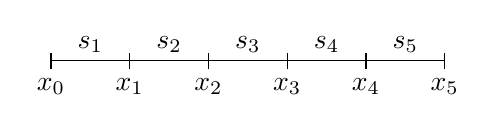
\begin{tikzpicture}
\draw (0,0) -- (5,0);
\foreach \x/\l in {.5cm/$s_1$, 1.5cm/$s_2$, 2.5cm/$s_3$, 3.5cm/$s_4$, 4.5cm/$s_5$}
  \node at (\x,2mm) {\l};
\foreach \x/\l in {0cm/$x_0$, 1cm/$x_1$, 2cm/$x_2$, 3cm/$x_3$, 4cm/$x_4$, 5cm/$x_5$}
  \draw (\x,-1mm) -- (\x,1mm) node[below,yshift=-2mm] {\l};
\end{tikzpicture}
\end{center}
and measure the distance and time for each segment individually. Then, we can compute the velocities for each segment. In symbols, if we denote the length of the segment $s_i$ by $\Delta s_i = x_{i+1}-x_i$ and the time it takes the robot to cross segment $s_i$ by $\Delta t_i = t_{i+1}-t_i$, then $v_i$, the velocity in segment $s_i$ is given by:
\[v_i = \frac{\Delta s_i}{\Delta t_i}\,.\]

Figure~\ref{fig.instant-v} is a graph of distance vs. time for an accelerating robot. The time axis has been divided into segments and the slopes $\displaystyle\frac{\Delta s_i}{\Delta t_i}$ show the average velocity in each segment which increases with time.

\begin{figure}
\begin{center}
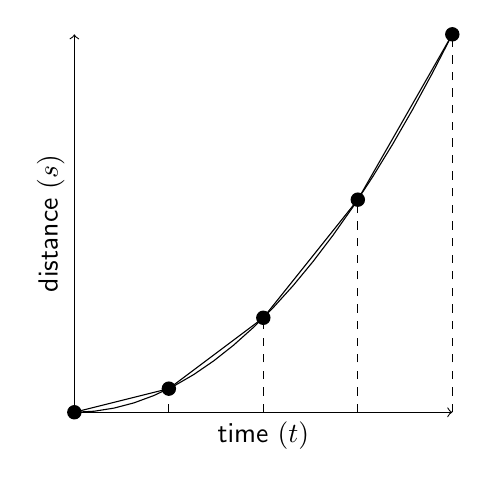
\begin{tikzpicture}[scale=1.2,samples=20,domain=0:4]
\draw[<->] (4,0) -- node[below] {\textsf{time} ($t$)} (0,0) -- node[sloped,above] {\textsf{distance} ($s$)} (0,4);
\draw plot (\x,{\x*\x/4});
\draw[mark=*] plot coordinates {(0,0) (1,.25) (2,1) (3,2.25) (4,4)};
\draw[dashed] (1,0) -- (1,.25);
\draw[dashed] (2,0) -- (2,1);
\draw[dashed] (3,0) -- (3,2.25);
\draw[dashed] (4,0) -- (4,4);
\end{tikzpicture}
\caption{An accelerating robot: distance increase as the square of time}\label{fig.instant-v}
\end{center}
\end{figure}

\emph{Acceleration} is defined as the change in velocity over a period of time:
\[a_i = \frac{\Delta v_i}{\Delta t_i}\,.\]
When the power setting of the robot is set to a fixed value, the force applied to the robot is constant and we expect that the acceleration remains constant, increasing the velocity. However, at a certain point the acceleration is reduced to zero, meaning that the velocity no longer increases, because the power applied to the wheels is just sufficient to overcome the friction of the road and the wind resistance.

Let us see what happens if the power setting is increased with time.

\begin{framed}
\act{Acceleration}{accel}
\begin{itemize}
\item Write a program that causes the robot to accelerate by increasing the power setting periodically. For example, start the robot at power $20$ and increase to $40$ after $1$ s, then to $60$ after $2$ s, to $80$ after $3$ s, and finally to $100$ after $4$ s.
\item Place the robot on the track and run the program.
\item Record the distances between each change of the power setting. Compute and plot the velocities in each of these segments.
\end{itemize}
\end{framed}

\section{From segments to continuous motion}\label{s.continuous}

As the size of the segments becomes smaller, we obtain the instantaneous velocity\index{velocity!instantaneous} of the robot at a single point in time, expressed as a derivative:
\[v(t) = \frac{ds(t)}{dt}\,.\]
Similarly, the instantaneous acceleration\index{acceleration!instantaneous} of the robot is defined as:
\[a(t) = \frac{dv(t)}{dt}\,.\]
For constant acceleration the velocity can be obtained by integrating the derivative:
\[v(t) = \int a\, dt = a\int {dt} = at\,,\]
and then the distance can be obtained by integrating again:
\[s(t) = \int v(t) dt=\int a\,t\,dt = \frac{at^2}{2}\,.\]

\noindent{}\textbf{Example} An average car accelerates from $0$ to $100$ km/h in about $10$ s. First, we convert units from km/h to m/s:
\[
v_{\textit{max}} = 100\, \textrm{km/h} = \frac{100\cdot 1000}{60\cdot 60} \,\textrm{m/s} = 27.8 \,\textrm{m/s}\,.
\]
Assuming constant acceleration, $v_{\textit{max}} = 27.8 = at = 10a$, so the acceleration is $2.78$ m/s$^{2}$ (read, $2.78$ meters per second per second, that is, every second the speed increases by $2.78$ meters per second). The distance the car moves in $10$ s is:
\[s(10) = \frac{at^2}{2} = \frac{2.78\cdot 10^2}{2}= 139 \,\textrm{m}\,.\]

\begin{framed}

\act{Computing distance when accelerating}{distance-a}
\begin{itemize}
\item For various vehicles (racing cars, motorcycles) look up the time required to accelerate from $0$ to $100$ km/h. Compute the distance moved.
\item Assume that the acceleration of a vehicle increases linearly, that is, $a=kt$ for a constant $k$. What are $v(t)$ and $s(t)$.
\item For several values of $k$ and $t$, compute the final velocities and distances.
\end{itemize}
\end{framed}

\begin{framed}
\act{Measuring motion at constant acceleration}{constant-a}
\begin{itemize}
\item Write a program that applies the maximum power setting to a robot.
\item Place the robot on a surface and run the program.
\item When the robot seems to have reached full speed record the time from the start of the run.
\item Compare the measured distance to $s = at^2/2$ (Fig.~\ref{fig.acc-distance}).
\item Run again and measure the distances at fixed intervals of time. Compute the speeds from the distances divided by the time and compare to $v=at$ (Fig.~\ref{fig.acc-velocity}).
\item In some robots you can set a target speed and read the actual speed. If your robot can do this, compare the measured speeds with the computed speeds.
\end{itemize}
\end{framed}

\begin{figure}
\subfigures
\begin{minipage}{\textwidth}
\leftfigure{
\begin{tikzpicture}[samples=20,domain=0:4]
\draw[<->] (4,0) -- node[below] {\textsf{time} ($t$)} (0,0) -- node[sloped,above] {\textsf{velocity} ($v$)} (0,4);
\draw plot (\x,{.5*\x});
\end{tikzpicture}
}
\hspace{\fill}
\rightfigure{
\begin{tikzpicture}[samples=20,domain=0:4]
\draw[<->] (4,0) -- node[below] {\textsf{time} ($t$)} (0,0) -- node[sloped,above] {\textsf{distance} ($s$)} (0,4);
\draw plot (\x,{.5*\x*\x/2});
\end{tikzpicture}
}
\leftcaption{Velocity for constant acceleration}\label{fig.acc-velocity}
\rightcaption{Distance for constant accleration}\label{fig.acc-distance}
\end{minipage}
\end{figure}

\section{Navigation by odometry}\label{s.odometry}
\index{odometry}

Suppose that you are in a car and your navigation system issues the following instruction: ``In 700 meters turn right.'' Now your task is very simple: Make observations of your car's odometer which measures how far you have traveled. When its value approaches 700 meters beyond its initial reading, look for a street on the right. An odometer in a car measures speed and time, and multiplies the two values to compute the distance traveled.

\emph{Odometry}---the measurement of distance---is a fundamental method used by robots for navigation. Measuring time is easy using the internal clock of the embedded computer. Measuring speed is more difficult: in some educational robots wheel encoders are used to count the rotations of the wheels (Sect.~\ref{s.wheel}), while in others speed is estimated from properties of the motors. From the distance moved $s=vt$, the new position of the robot can be computed. In one dimension, the computation is trivial, but it becomes a bit more complex when the motion involves turns. This section presents the computation of distance by odometry, first for a robot moving linearly and then for a robot making a turn.

Section~\ref{s.odometry-errors} shows how errors in heading are more serious than errors in distance.

A disadvantage of odometry (with or without wheel encoders) is that the measurements are indirect, relating the power of the motors or the motion of the wheels to changes in the robot's position. This can be error-prone since the relation between motor speed and wheel rotation can be very nonlinear and vary with time. Furthermore, wheels can slip and skid so there may be errors in relating the motion of the wheels to the the motion of the robot. Improved estimates of position can be obtained by using an inertial navigation system, which directly measures acceleration and angular velocity that can be used to determine the robot's position (Sect.~\ref{s.imu}).

Odometry is a form of \emph{localization}: the robot must determine its position in the environment. In odometry we determine position by measuring the change from the robot's known initial position, while localization (Chap.~\ref{ch.local}) refers to the determination of the position of a robot relative to the known positions of other objects such as landmarks or beacons.


\section{Linear odometry}
\index{odometry!linear}

Before studying the mathematics of odometry you should try the following Activity:

\begin{framed}
\act{Distance from speed and time}{odometry1}
\begin{itemize}
\item Run the robot at a constant power setting for a specific period of time and measure the distance moved.
\item Repeat the measurement several times. Is the distance constant? If not, how much does it vary as a percentage of the distance?
\item Repeat the measurement several times for different power settings. Is the distance measured linear in the power setting? Does the \emph{variation} in the distance measurement on multiple runs depend on the power setting?
\item Repeat the measurement for a fixed power setting but for different periods of time and analyze the results.
\end{itemize}
\end{framed}

When a relation between motor power and velocity $v$ has been determined, the robot can compute the distance moved by $s=vt$. If it starts at position $(0,0)$ and moves straight along the $x$-axis, then after $t$ seconds its new position is $(vt,0)$.

This activity should demonstrate that it is possible to measure distance by odometry with reasonable precision and accuracy. A self-driving car can use odometry to determine its position so that it doesn't have to analyze its sensor data continuously to check if the required street has been reached. Given the uncertainties of motion and of the road, the car should not depend only on odometry to decide when to turn, but the error will not be large and the sensor data can be analyzed to detect the turn when odometry indicates that the car is in the vicinity of the intersection.

Activity~\ref{act.odometry1} asked you to measure the distance moved in one dimension. Three items of information need to be computed if the motion is in two dimensions: the robot's \emph{position} $(x,y)$ relative to a fixed origin and its \emph{heading} $\theta$, the direction in which the robot is pointing (Fig.~\ref{fig.pos-head}). The triple $(x,y,\theta)$ is called the \emph{pose}\index{pose} of the robot. If the robot starts at the origin $(0,0)$ and moves in a straight line at angle $\theta$ with velocity $v$ for time $t$, the distance moved is $s=vt$. Its new position $(x,y)$ is:
\begin{eqnarray*}
x &=& vt \cos \theta\\
y &=& vt \sin \theta\,.
\end{eqnarray*}

\begin{figure}
\begin{center}
\begin{tikzpicture}[scale=1.2]
\draw (-1,0) -- (4,0);
\draw (0,-1) -- (0,3);
\node at (-5mm,-4mm) { $(0,0)$ };
\pic[rotate=30,scale=.6] at (0,0) { robot };
\pic[rotate=30,scale=.6] at (30:3) { robot };
\draw[dashed] (30:3) -| (0,0);
\draw[dashed] (30:3) |- (0,0);
\node at (1.2,1.7) {$x$};
\node at (2.8,.5) {$y$};
\draw[->] (30:3) -- +(30:1.2) {};
\draw[->] (0,0) -- +(30:1.2) {};
\node at (1,.3) {$\theta$};
\end{tikzpicture}
\caption{Position and heading}\label{fig.pos-head}
\end{center}
\end{figure}

\section{Odometry with turns}\label{s.odometry-turns}
\index{odometry!turns@with turns}

Suppose that the robot turns slightly left because the right wheel moves faster than the left wheel (Fig.\ref{fig.small-turn}). In the figure, the robot is facing towards the top of the page; the blue dot is the left wheel, the red dot is the right wheel, and the black dot is the center of the robot which is halfway between the wheels. The \textit{baseline} $b$ is the distance between the wheels, and $d_l, d_r, d_c$ represent the distances moved by the two wheels and the center when the robot turns. We want to compute the new position and heading of the robot.

We can measure $d_l$ and $d_r$, the distances moved by the two wheels using the method described in Activity~\ref{act.odometry1}: relating motor power to rotational speed and then multiplying by time. Alternatively, we can use the number of rotations counted by the wheel encoders. If the radius of a wheel is $R$ and the rotational speeds of the left and right wheels are $\omega_l,\omega_r$ revolutions per second, respectively, then after $t$ seconds the wheel has moved:
\begin{equation}
d_i=2\pi R \omega_i t,\;\;\; i=l,r\,. \label{eq.rotation}
\end{equation}
The task is to determine the new pose of the robot after the wheels have moved these distances.

\begin{figure}
\begin{center}
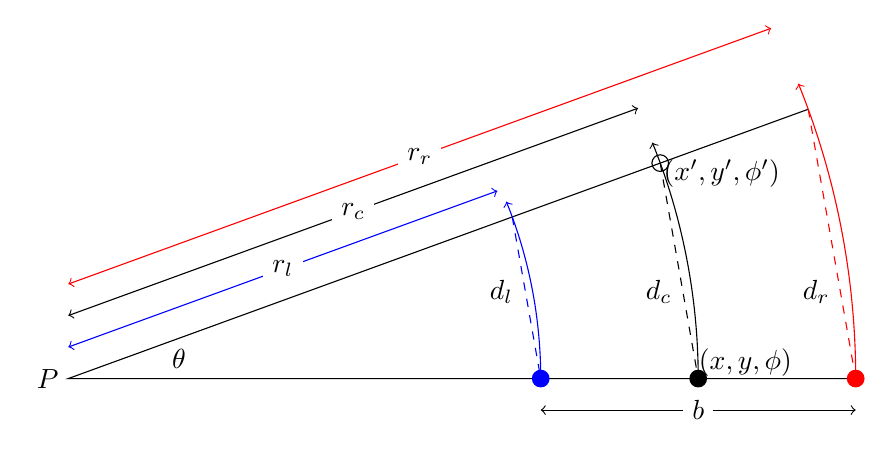
\begin{tikzpicture}
% Draw angle lines
\draw (10,0) -- %
  (0,0) coordinate(origin) node [right=40pt,above] {$\theta$} -- %
  (20:10);
\node[left] at (0,0) {$P$};
% Arrows with baseline
\draw[<->] (6,-.4) -- %
  node[fill=white] {$b$} (10,-.4);
% Three: large dots, arcs, dashed lines, labels
\foreach \x/\d/\c in {6/$d_l$/blue,8/$d_c$/black,10/$d_r$/red}
{
  \draw[dashed,\c] (20:\x) -- (\x,0);
  \draw[->,\c] (\x,0) arc (0:22:\x);
  \node at (\x-.5,1.1) {\d};
  \draw[fill,\c] (\x,0) circle[radius=3pt];
}
\draw[<->,blue] (0,4mm) -- node[black,fill=white] {$r_l$} +(20:58mm);
\draw[<->,black] (0,8mm) -- node[black,fill=white] {$r_c$} +(20:77mm);
\draw[<->,red] (0,12mm) -- node[black,fill=white] {$r_r$} +(20:95mm);
\node at (8.6,.2) {$(x,y,\phi)$};
\node at (8.3,2.6) {$(x',y',\phi')$};
\draw (20:8) circle[radius=3pt];
\end{tikzpicture}
\end{center}
\caption{Geometry of a left turn by a robot with two wheels}\label{fig.small-turn}
\end{figure}

Figure\ref{fig.small-turn} shows the robot initially at pose $(x,y,\phi)$, where the robot is facing north ($\phi=\pi/2$). After turning $\theta$ radians, what is the new pose $(x',y',\phi')$? Clearly, the heading of the robot is now $\phi'=\phi+\theta$, but we also have to compute $x',y'$.

The length of an arc of angle $\theta$ radians is given by its fraction of the circumference of the circle: $2\pi r\,(\theta/2\pi)=\theta r$. For small angles, the distances $d_l,d_c,d_r$ are approximately equal to the length of the corresponding arcs, so we have:
\begin{eqnarray}
\theta &=& d_l/r_l = d_c/r_c = d_r/r_r\,,\label{eqn.theta}
\end{eqnarray}
where $r_l, r_r, r_c$ are the distances from $P$, the origin of the turn.

The distances $d_l$ and $d_r$ are obtained from the rotations of the wheels (Eq.~\ref{eq.rotation}) and the baseline $b$ is a fixed physical measurement of the robot. From Eq.~\ref{eqn.theta}, the angle $\theta$ can be computed:
\begin{eqnarray*}
\theta r_r &=& d_r\\
\theta r_l &=& d_l\\
\theta r_r - \theta r_l &=& d_r - d_l\\
\theta &=& (d_r - d_l) / (r_r - r_l)\\
\theta &=& (d_r - d_l) / b\,.
\end{eqnarray*}
The center is halfway between the wheels $r_c =(r_l+r_r)/2$,
so again by Eq.~\ref{eqn.theta}:
\begin{eqnarray*}
d_c&=&\theta r_c\\
&=&\theta \left(\frac{r_l+r_r}{2}\right)\\
&=&\frac{\theta}{2} \left(\frac{d_l}{\theta} + \frac{d_r}{\theta}\right)\\
&=&\frac{d_l+d_r}{2}\,.
\end{eqnarray*}

If the distance moved is small, the line labeled $d_c$ is approximately
perpendicular to the radius through the final position of the robot. By similar triangles, we see that $\theta$ is the change in the heading of the robot (Fig.~\ref{fig.heading}). By trigonometry:\footnote{You were probably expecting $\cos$ for $dx$ and $\sin$ for $dy$. That would be the case if the robot were facing along the $x$ axis. However, the initial pose is $\phi=\pi/2$ and we have $\sin(\theta+\pi/2)=\cos\theta$ and $\cos(\theta+\pi/2)=-\sin\theta$.}
\begin{eqnarray*}
\textit{dx} &=& - d_c \sin \theta\\
\textit{dy} &=& d_c \cos \theta\,,
\end{eqnarray*}
so the pose of the robot after the turn is:
\[
(x',y',\phi') = ( - d_c \sin \theta, d_c \cos \theta, \phi+\theta)\,.
\]

\begin{figure}
\begin{center}
\begin{tikzpicture}
% Draw angle with thetas
\draw (10,0) coordinate (A) -- %
  (0,0) coordinate (origin) node [right=40pt,above] {$\theta$} -- %
  (20:9) coordinate (B) node [xshift=1.5mm,yshift=-7mm] {$\theta$};
% Dashed line to complete the triangle
\draw[dashed] (A) -- node [right=1pt] {$d_c$} (B);
% Dashed perpendicular lines
\draw[dashed] (B) -- node [left] {$d_y$} ({B} |- {A}) coordinate (C);
\draw[dashed] (A) node[above left,xshift=1pt,yshift=14pt] {$\theta$} -- (A |- B);
% Dummy line for placing dx label
\path (C) -- node [below=1pt] {$d_x$} (A);
% Rectangles for right angles
\draw (C) rectangle +(6pt,6pt);
\draw[rotate=20] (B) rectangle +(-6pt,-6pt);
\end{tikzpicture}
\end{center}
\caption{Change in heading}\label{fig.heading}
\end{figure}

The formulas show how to compute the changes \textit{dx}, \textit{dy} and $\theta$ when the robot moves a short distance. To compute odometry over longer distances, this computation must be done frequently. There are two reasons why the intervals between the computations must be short: (a) the assumption of constant speed holds only for short distances, and (b) the trigonometric calculation is simplified by assuming that the distance moved is short.

\begin{framed}
\act{Odometry in two dimensions}{odometry2}
\begin{itemize}
\item Write a program that causes the robot to make a gentle left turn for a specific period of time.
\item Compute the pose $( - d_c \sin \theta, d_c \cos \theta, \theta)$ and compare the result with the values measured using a ruler and a protractor. Run the program several times and see if the measurements are consistent.
\item Run the program for different periods of time. How does this affect the accuracy and precision of the odometry computation?
\end{itemize}
\end{framed}

\section{Errors in odometry}\label{s.odometry-errors}

We have already noted that odometry is not accurate because inconsistent measurements and irregularities in the surface can cause errors. In this section we show that even small changes in the direction of the robot's movement can cause errors that are much larger than those caused by changes in its linear motion.

To simplify the presentation, let us assume that a robot is to move $10$ meters from the origin of a coordinate system along the $x$-axis and then check its surroundings for a specific object. What is the effect of an error of \emph{up to} $p\,\%$? If the error is in the measurement of $x$, the distance moved, then $\Delta x$, the error in $x$ is:
\[\Delta x \leq \pm 10\cdot\frac{p}{100} = \pm\frac{p}{10}\; \textrm{meter}\,,\]
where the value is negative or positive because the robot could move up to $p\,\%$ before or after the intended distance.

Suppose now that there is an error $p\%$ in the \emph{heading} of the robot, and, for simplicity, assume that there is no error in the distance moved. The geometry is:
\begin{center}
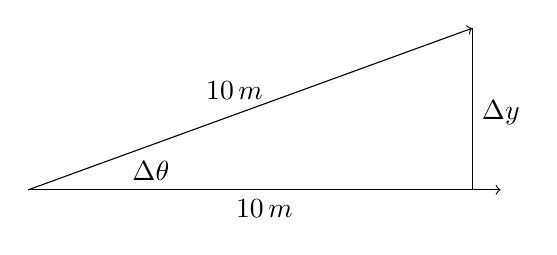
\begin{tikzpicture}
\draw[->] (0,0) -- node[below] {$10\,m$} (6,0);
\draw[->] (0,0) -- node[above,xshift=-2mm] {$10\,m$} +(20:6);
\draw (20:6) |- node[above right,yshift=7mm] {$\Delta y$} (0,0);
\node[above right,xshift=12mm] at (0,0) {$\Delta \theta$};
\end{tikzpicture}
\end{center}
The robot intended to move $10$ m along the $x$-axis, but instead it moved slightly to the left at an angle of $\Delta \theta$. Let us compute the left-right deviation $\Delta y$. By trigonometry, $\Delta y = 10\sin \Delta\theta$. An error of $p\,\%$ in heading is:
\[
\Delta\theta=360\cdot\frac{p}{100}=(3.6p)^\circ\,,
\]
so the left-right deviation is:
\[
\Delta y \leq \pm 10 \sin (3.6p)\,.
\]

The following tables compare the difference between a linear error of $p\,\%$ (left) and an error in heading of $p\,\%$ (right):
\begin{displaymath}
\setlength{\arraycolsep}{2ex}
\renewcommand{\arraystretch}{1.1}
\begin{array}{r|r}
\svhline\noalign{\smallskip}
\multicolumn{1}{c|}{p\,\%} & \multicolumn{1}{c}{\Delta x \,(m)}\\
\noalign{\smallskip}\svhline\noalign{\smallskip}
1 & .1 \\
2 & .2 \\
5 & .5 \\
10 & 1.00\\
\noalign{\smallskip}\svhline\noalign{\smallskip}
\end{array}
\;\;\;\;\;\;\;\;
\begin{array}{r|rrr}
\svhline\noalign{\smallskip}
\multicolumn{1}{c|}{p\,\%} & \multicolumn{1}{c}{\Delta \theta\,({}^\circ)} & \multicolumn{1}{c}{\sin\Delta\theta} & \multicolumn{1}{c}{\Delta y \,(\textrm{m})}\\
\noalign{\smallskip}\svhline\noalign{\smallskip}
1 &  3.6 & .063 & .63\\
2 &  7.2 & .125 & 1.25\\
5 &  18.0 & .309 & 3.09\\
10 & 36.0 & .588 & 5.88\\
\noalign{\smallskip}\svhline\noalign{\smallskip}
\end{array}
\end{displaymath}

For a very small error like $2\,\%$, the distance error after moving $10$ m is just $.2$ m, which should put the robot in the vicinity of the object it is searching for, but a heading error of the same percentage places the robot $1.25$ m away from the object. For a more significant error like $5\,\%$ or $10\,\%$, the distance error ($50$ cm or $100$ cm) is still possibly manageable, but the heading error places the robot $3.09$ m or $5.88$ m away, which is not even in the vicinity of the object.

The accumulation of odometry errors as the distance moved gets longer is displayed in Fig.~\ref{fig.odo-errors}. The initial position of the robot is denoted by the dot at the origin.  Assuming an error of at most $\pm 4\,\%$ in both the linear direction and the heading, the possible positions of the robot after moving $d=1,2,\ldots,10$ meters are displayed as ellipses. The minor radii of the error ellipses result from the linear errors:
\[.04s = 0.04, .08, \ldots, .4 \;\;\textrm{meters},
\]
while the major radii of the error ellipses result from the angular errors:
\[
d\sin \,(.04\cdot 360^\circ)=d \sin 14.4^\circ \approx{} .25, .50, \ldots 2.5\;\;\textrm{meters}.
\]
Clearly, the angular errors are much more significant than the linear errors.

\begin{figure}
\begin{center}
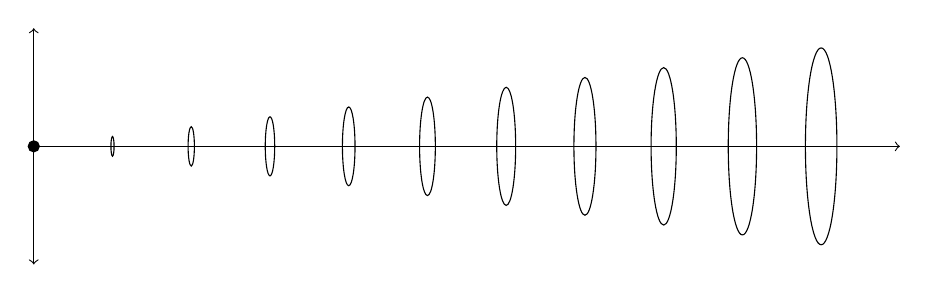
\begin{tikzpicture}
\draw[<->] (0,1.5) -- (0,-1.5);
\draw[->] (0,0) -- (11,0);
\draw[fill](0,0) circle[radius=2pt];
\foreach \x/\mult in {1/1, 2/2, 3/3, 4/4, 5/5, 6/6, 7/7, 8/8, 9/9, 10/10}
  \draw (\x,0) ellipse [x radius=\mult*.02cm, y radius=\mult*.125cm];
\end{tikzpicture}
\end{center}
\caption{Odometry errors}\label{fig.odo-errors}
\end{figure}

Since error is unavoidable, periodically the pose of the robot as computed by odometry must be compared with an absolute position; this becomes the new initial position for further computation. Methods for determining the absolute position of the robot are presented in Chap.~\ref{ch.local}.

\begin{framed}
\act{Odometry errors}{odo-error}
\begin{itemize}
\item Write a program to cause the robot to move in a straight line for $2$ meters. Make sure that the surface is smooth so that it doesn't turn off course and calibrate the motor settings so that the robot moves as straight as possible.
\item Vary the motor power of both wheels together so that the robot runs somewhat slower or somewhat faster than before. Plot its position at fixed intervals and see if the error remains linear over the course.
\item Vary the motor power of one wheel so that the robot turns slightly to one side. Plot its position at fixed intervals and see if the errors are proportional to the sine of the difference between the original heading and the new heading.
\end{itemize}
\end{framed}

\begin{framed}
\act{Combined effect of odometry errors}{odo-combine}
\begin{itemize}
\item Write a program that causes the robot to move in a straight line for $2$ meters and then turn $360^\circ$. What is the error in the robot's position?
\item Write a program that causes the robot to turn $360^\circ$ and then move in a straight line for $2$ meters. What is the error in the robot's position? Is there a difference between this error and the error of the previous experiment?
\item Write a program that causes the robot to move in a straight line for $2$ meters, turn $180^\circ$ and then move in a straight line for $2$ meters. How far is it from its starting position?
\end{itemize}
\end{framed}

\begin{framed}
\act{Correcting odometry errors}{odo-correct}
\begin{itemize}
\item Modify the program that you wrote for Activity~\ref{act.odo-error} to introduce \emph{jitter}, random variation in the power supplied to the motor. Check that the distance that the robot moves in a fixed time is not constant, but changes slightly from run to run.
\item Mark a goal line on the floor and compute the time it should take the robot to reach the goal.
\item When the robot has moved for that period of time, see if it can find the goal by moving forwards and backwards in small steps until it detects the goal.
\end{itemize}
\end{framed}


\section{Wheel encoders}\label{s.wheel}
\index{wheel encoder}

Odometry in a wheeled vehicle like a car can be improved by measuring the rotation of the wheels instead of mapping motor power into velocity. The circumference of a wheel is $2\pi r$, where $r$ is the radius of the wheel in cm, so if $n$ rotations are counted, we know that the robot has moved $2\pi n r$ cm. Wheel encoders can be built that measure fractions of a revolution. If a signal is generated $8$ times per revolution, the distance moved is $2\pi nr /8$ cm, which $n$ is now the number of signals counted by the computer.

There are many different ways of implementing wheel encoders. A popular design is to use a light source such as a light-emitting diode (LED), a light sensor and an encoding disk that is attached to the axis of the wheel (Fig.~\ref{fig.wheel}). The disk is perforated with holes (Fig.~\ref{fig.encoding-disk}) so that whenever the hole is opposite the light source, the sensor generates a signal.

\begin{figure}
\subfigures
\begin{minipage}{\textwidth}
\leftfigure[c]{
\begin{tikzpicture}[scale=.7]
% Draw axle
\draw[thick,fill=gray!80] (0,-.18) rectangle (5,.18) node[right=4pt,yshift=10pt,text width=8mm] {\textsf{to motor}};
% Draw disk
\draw[rounded corners,fill=gray!10] (3,-1.6) node[right=10pt,yshift=3pt] {\textsf{encoding disk}} rectangle +(.4,3.2);
% Draw wheel
\draw[rounded corners,thick,fill=gray!20] (0,-2) to [bend left=10] (0,2) node[xshift=3.5mm,yshift=3mm] {\textsf{wheel}} -- (1,2) to [bend left=10](1,-2) -- cycle;
\begin{scope}[xshift=20mm,yshift=8mm]
% LED
\draw[red] (0,0) rectangle node[black,above=12pt] {\textsf{LED}} (.3,.6);
\draw[red,bend right=90] (.3,0) to (.3,.6);
% Sensor
\draw[blue] (2,0) rectangle node[black,above=12pt] {\textsf{sensor}} (2.3,.6);
\draw[blue,bend left=90] (2,0) to (2,.6);
\end{scope}
\draw[raxis] (-15mm,0) -- (64mm,0);
\end{tikzpicture}
}
\hspace{\fill}
\rightfigure[c]{
\begin{tikzpicture}[scale=.5,baseline=-14mm]
\draw[fill=gray!20] (0,0) circle [radius=25mm];
\draw[fill=white] (0,0) circle [radius=5mm];
\foreach \x/\y/\theta in {
  0/18/0, 0/-18/0, 18/0/90, -18/0/90,
  12.5/12.5/-45, -12.5/12.5/45, 12.5/-12.5/-135, -12.5/-12.5/135
} {
  \node [draw,fill=white,shape=rectangle,inner sep=0pt,minimum width=3mm,minimum height=5mm,anchor=center,rotate=\theta] at (\x mm,\y mm) {};
}
\draw[raxis] (0,0) -- (10pt,0);
\draw[raxis] (0,0) -- (-10pt,0);
\draw[raxis] (0,0) -- (0,10pt);
\draw[raxis] (0,0) -- (0,-10pt);
\end{tikzpicture}
}
\leftcaption{Optical wheel encoder\label{fig.wheel}}
\rightcaption{Encoding disk\label{fig.encoding-disk}}
\end{minipage}
\end{figure}

The support for wheel encoders in educational robots varies:
\begin{itemize}
\item If a robot does not have wheel encoders it must be calibrated;
\item The robot may have wheel encoders that are used internally;
\item Some robots like the \lego{} Mindstorms enable the user to read the encoders.
\end{itemize}
The following activity proposes an experiment to measure the distance moved by counting revolutions of a wheel. It can be carried out even if your robot does not have wheel encoders or they are not accessible.

\begin{framed}
\act{Wheel encoding}{wheel}
\begin{itemize}
\item Make a mark at the top of a wheel of the robot using chalk or by attaching a narrow piece of colored tape. Write a program that causes the robot to move straight ahead for a fixed period of time. Run the program and take a video of the side of the robot using the camera on your smartphone.
\item View the video and determine the number of revolutions by counting the number of times the mark is at the top of the wheel.
\item Measure the radius of the wheel and compute the distance moved. How close is the result to the actual distance measured on the floor?
\item Repeat the measurement using $n=2$ and then $n=4$ equally spaced marks on the wheel. Determine the number of revolutions by counting the number of times that a mark is at the top of the wheel and divide by $n$. Compute the distance.
\end{itemize}
\end{framed}

\section{Inertial navigation systems}\label{s.imu}
\index{inertial navigation system}

An \emph{inertial navigation system (INS)} directly measures linear acceleration and angular velocity and uses them to calculate the pose of a vehicle. The term \emph{inertial measurement unit (IMU)} is also used, but we prefer the term INS which refers to the entire system. Integrating acceleration from the initial pose to the current time $\tau$ gives the current velocity:
\[
v=\int_0^\tau a(t) \,dt\,.
\]
Similarly, integrating angular velocity gives the change in heading:
\[
\theta = \int_0^\tau \omega(t) \, dt\,.
\]
In an INS, we are not given continuous functions to integrate; instead, the acceleration and angular velocity are sampled and summation replaces integration:
\[
v_n = \sum^{n}_{i=0} a_n \Delta t,\;\; \theta_n = \sum^{n}_{i=0} \omega_n \Delta t\,.
\]
INSs are subject to errors caused by inaccuracies in the measurement itself as well as by variations caused by environmental factors such as temperature, and by wear and tear of the unit. Inertial measurement is often combined with GPS (Sect.~\ref{s.gps}) to update the position with an absolute location.

INSs for robots are constructed with \emph{microelectromechanical systems (MEMS)}\index{microelectromechanical systems}, which use integrated circuit manufacturing techniques that combine mechanical elements with electronics that interface with the robot's computer.

\subsection{Accelerometers}\label{s.accelerometer}
\index{inertial navigation system!accelerometer}

If you have ever flown on an airplane you have experienced a force pushing you back into your seat as a result of the rapid acceleration of the airplane upon takeoff. Upon landing you are pushed away from your seat. You can also experience this in a car that accelerates rapidly or makes an emergency stop. Acceleration is related to force by Newton's second law $F=ma$, where $m$ is the mass. By measuring the force on an object, we measure the acceleration.

Figures~\ref{fig.acc-forward}--\ref{fig.acc-backward} show how an accelerometer can be built from an object (called a \emph{mass}) connected to a spring. The greater the acceleration, the greater the force exerted by the mass upon the spring, which in turn causes the spring to be compressed. The direction that the mass moves gives the sign of the acceleration: forwards or backwards. The magnitude of the force is measured indirectly by measuring the distance that the mass moves. You can see that the diagrams correspond to our experience: when a car accelerates, you are pushed back into the seat, but when it decelerates (brakes) you continue forward.

\begin{figure}
\subfigures
\leftfigure{
\begin{tikzpicture}
\draw[->] (-40mm,17mm) -- node[w,midway] {\p{front of vehicle}} (-8mm,17mm);
\draw (2mm,14mm) -- (-52mm,14mm) -- (-52mm,6mm) -- (2mm,6mm) -- cycle;
\draw (-50mm,10mm) -- (-52mm,10mm);
\draw (-50mm,10mm) -- ++(1mm,2mm) -- ++(1mm,-4mm) -- ++(1mm,4mm)  -- ++(1mm,-4mm) -- ++(1mm,4mm)  -- ++(1mm,-4mm) -- ++(1mm,4mm)  -- ++(1mm,-4mm) -- ++(1mm,4mm)  -- ++(1mm,-2mm) -- (-36mm,10mm);
\draw[fill] (-36mm,10mm) circle[radius=3mm];
\draw (0mm,10mm) -- (2mm,10mm);
\draw (0mm,10mm) -- ++(-3mm,2mm) -- ++(-3mm,-4mm) -- ++(-3mm,4mm)  -- ++(-3mm,-4mm) -- ++(-3mm,4mm)  -- ++(-3mm,-4mm) -- ++(-3mm,4mm)  -- ++(-3mm,-4mm) -- ++(-3mm,4mm)  -- ++(-3mm,-2mm) -- (-36mm,10mm);
\end{tikzpicture}
}
\hspace{\fill}
\rightfigure{
\begin{tikzpicture}[rotate=180]
\draw[<-] (-40mm,3mm) -- node[w,midway] {\p{front of vehicle}} (-8mm,3mm);
\draw (2mm,14mm) -- (-52mm,14mm) -- (-52mm,6mm) -- (2mm,6mm) -- cycle;
\draw (-50mm,10mm) -- (-52mm,10mm);
\draw (-50mm,10mm) -- ++(1mm,2mm) -- ++(1mm,-4mm) -- ++(1mm,4mm)  -- ++(1mm,-4mm) -- ++(1mm,4mm)  -- ++(1mm,-4mm) -- ++(1mm,4mm)  -- ++(1mm,-4mm) -- ++(1mm,4mm)  -- ++(1mm,-2mm) -- (-36mm,10mm);
\draw[fill] (-36mm,10mm) circle[radius=3mm];
\draw (0mm,10mm) -- (2mm,10mm);
\draw (0mm,10mm) -- ++(-3mm,2mm) -- ++(-3mm,-4mm) -- ++(-3mm,4mm)  -- ++(-3mm,-4mm) -- ++(-3mm,4mm)  -- ++(-3mm,-4mm) -- ++(-3mm,4mm)  -- ++(-3mm,-4mm) -- ++(-3mm,4mm)  -- ++(-3mm,-2mm) -- (-36mm,10mm);
\end{tikzpicture}
}
\leftcaption{Forward acceleration}\label{fig.acc-forward}
\rightcaption{Deceleration (braking)}\label{fig.acc-backward}
\end{figure}

\subsection{Gyroscopes}
\index{inertial navigation system!gyroscope}

A \emph{gyroscope} (``gyro'') uses the principle of Coriolis force to measure angular velocity. This concept is explained in textbooks on physics and we will not go into it here. There are many types of gyros:
\begin{itemize}
\item Classical gyros have spinning mechanical disks which are mounted on gimbals so that the axis of rotation remains fixed in space. These gyros are extremely accurate but are very heavy and consume a lot of power. They are found on high-value vehicles such as aircraft and rockets.
\item Ring laser gyros (RLG) have (almost) no moving parts and are preferred over mechanical gyros for most applications. They are based on sending two laser beams in opposite directions around a circular or triangular path. If the gyro is rotating, the path followed by one laser beam will be longer than the path followed by the other beam. The difference is proportional to the angular velocity and can be measured and transfered to the navigation computer.
\item Coriolis vibratory gyroscopes (CVG) manufactured using MEMS techniques are found in smartphones and robots. They are inexpensive and extremely robust, although their accuracy is not as good are the gyros previously discussed. We now give an overview of how they work.
\end{itemize}

Figure~\ref{fig.tuning-gyro-image} shows a CVG called a \emph{tuning fork gyroscope}. Two square masses are attached by flexible beams to anchors that are mounted on the base of the component. Drivers force the masses to vibrate left and right. If the component rotates, the masses move upwards and downwards a distance proportional to the angular velocity. The masses and the electrodes form the plates of capacitors whose capacitance increases or decreases as the plates come together or move apart.

\begin{figure}
\begin{center}
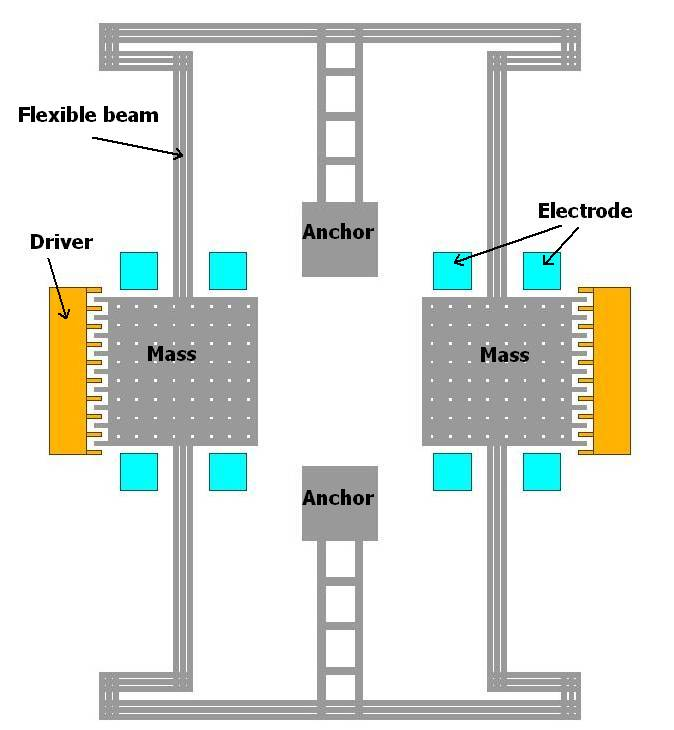
\includegraphics[width=.7\textwidth]{tuning-fork-gyro}
\end{center}
\caption{Tuning fork gyroscope (Courtesy of Zhili Hao, Old Dominion University)}\label{fig.tuning-gyro-image}
\end{figure}

The theory of operation of the tuning fork gyroscope is shown in Fig.~\ref{fig.tuning-gyro}. The masses (gray squares) are forced to vibrate at the same frequency like the two prongs of a tuning fork. They vibrate in different directions, that is, they either approach each other (blue dotted arrows) or they move away from each other (dashed red arrows). The component rotates around an axis perpendicular to its center (the circle with a cross denotes the rotational axis which is perpendicular to the plane of the paper). The Coriolis force is a force whose direction is given by the vector cross product of the axis of the rotation and the movement of the mass, and whose magnitude is proportional to the linear velocity of the mass and the angular velocity of the gyro. Since the masses are moving in different directions, the resulting forces will be equal but in opposite directions (solid arrows). The masses approach or recede from the electrodes (small rectangles) and the change in capacitance can be measured by a circuit.

\begin{figure}
\begin{center}
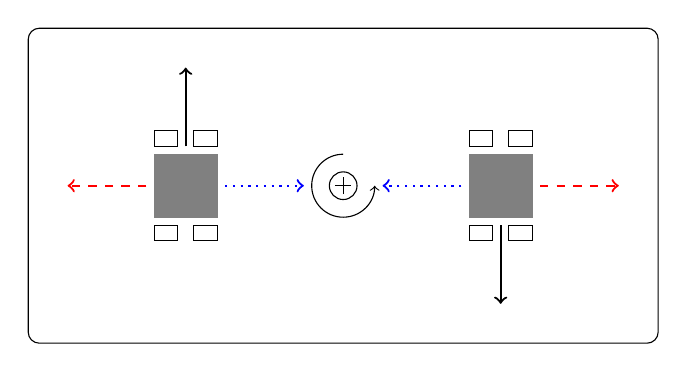
\begin{tikzpicture}
\draw[thin,rounded corners] (-4,-2) -- (4,-2) -- (4,2) -- (-4,2) -- cycle;
\draw[fill,gray] (-24mm,-4mm) rectangle +(8mm,8mm);
\draw[->,thick,dotted,blue] (-15mm,0mm) -- (-5mm,0mm);
\draw[->,thick,dashed,red] (-25mm,0mm) -- (-35mm,0mm);
\draw[->,thick] (-2,5mm) -- (-2,15mm);
\draw[fill,gray] (16mm,-4mm) rectangle +(8mm,8mm);
\draw[->,thick,dotted,blue] (15mm,0mm) -- (5mm,0mm);
\draw[->,thick,dashed,red] (25mm,0mm) -- (35mm,0mm);
\draw[->,thick] (2,-5mm) -- (2,-15mm);
\draw (0,0) circle[radius=5pt];
\draw (-3pt,0) -- (3pt,0);
\draw (0,-3pt) -- (0,3pt);
\draw[<-] (4mm,0) arc [start angle=0, end angle=-270, radius=4mm];
\foreach \x/\y in {-24/5,-19/5,16/5,21/5,-24/-7,-19/-7,16/-7,21/-7} {
  \draw (\x mm, \y mm) rectangle +(3mm,2mm);
}
\end{tikzpicture}
\end{center}
\caption{Physics of a tuning fork gyroscope: red dashed arrows and blue dotted arrows indicate the direction of the vibration; solid black arrows indiate the direction of the Coriolis force}\label{fig.tuning-gyro}
\end{figure}

\subsection{Applications}

An inertial navigation system has three accelerometers and three gyroscopes so that the pose of the vehicle can be computed in three dimensions. This is necessary for robotic aircraft and and other robotic vehicles. Airbags use an accelerometer that detects the rapid deceleration in the front-back direction that occurs when a car crashes. This causes an explosive expansion of the airbag. One can conceive of more applications for these components in cars. An accelerometer in the up-down direction can detect if the car has fallen into a pothole. A gyroscope measuring rotation around the vertical axis can detect skidding, while the gyroscope measuring rotation around the front-rear axis can detect if the car is rolling over.

%%%%%%%%%%%%%%%%%%%%%%%%%%%%%%%%%%%%%%%%%%%%%%%%%%%%%%%%%%%

\section{Degrees of freedom and numbers of actuators}\label{s.dof}
\index{degree of freedom}
\index{actuator}

The number of \emph{degrees of freedom (DOF)} of a system is the dimensionality of the coordinates needed to describe a pose of a mobile robot or the pose of the end effector of a robotic manipulator.\footnote{This section and the following ones are more advanced and can skipped during your first reading. Furthermore, some of the examples are of robotic manipulators described in Chap.~\ref{ch.kinematics}.} For example, a helicopter has six DOF because it can move in the three spatial dimensions and can rotate around the three axes. Therefore, a six-dimensional coordinate $(x,y,z,\phi,\psi,\theta)$ is needed to describe its pose.

\begin{quote}
\begin{center}
\textbf{The terms used to describe rotations}
\end{center}
A helicopter can rotate around all three of its axes. The rotations are called: (a) pitch: the nose moves up and down; (b) roll: the body rotates around its lengthwise axis; (c) yaw: the body rotates left and right around the axis of its rotor.
\end{quote}

The two-link robotic arm in Fig.~\ref{fig.two-link} has only two DOF because its end effector moves in a plane and does not rotate; therefore, it can be described by a two-dimensional coordinate $(x,y)$. By examining Fig.~\ref{fig.pos-head} again, you can see that a mobile robot moving on a flat surface has three DOF, because its pose is defined by a three-dimensional coordinate $(x,y,\theta)$. A train has only one DOF since it is constrained by the tracks to move forwards (or occasionally backwards) along the track. It only takes one coordinate $(x)$, the train's distance from an arbitrary origin of the track, to specify the pose of the train.

\begin{figure}
\begin{center}
% Forward kinematics
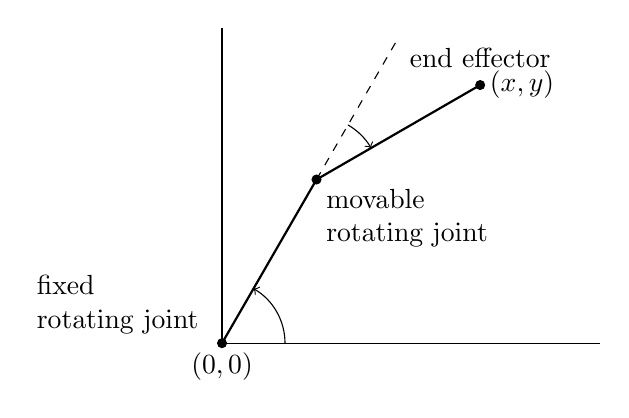
\begin{tikzpicture}[scale=.8,align=left]
\draw (0,0) coordinate (origin) -- (6,0);
\draw (origin) -- (0,5);
\draw[thick] (origin) -- ++(60:3) coordinate (prime) -- ++(30:3) coordinate (point);
\path (origin) -- ++(60:3) -- ++(30:1) coordinate (angle);
\draw[dashed] (60:3) -- ++(60:2.6);
\draw[->] (1,0) arc (0:60:1);
\draw[<-] (angle) arc (30:60:1);
\draw[fill] (origin) circle [radius=2pt] node[below] {$(0,0)$};
\draw[fill] (prime) circle [radius=2pt];
\draw[fill] (point) circle [radius=2pt] node[right] {$(x,y)$};
\node[above,yshift=1mm] at (point) {\p{end effector}};
\node[above left,xshift=-5pt] at (origin) {\p{fixed}\\\p{rotating joint}};
\node[below right] at (prime) {\p{movable}\\\p{rotating joint}};
\end{tikzpicture}
\end{center}
\caption{A two-link robotic arm with two DOF}\label{fig.two-link}
\end{figure}

We need more information than the degrees of freedom to describe robotic motion. Consider a vehicle like a car, a bicycle or an office chair. Although three coordinates $(x,y,\theta)$ are needed to describe its pose, we cannot necessarily move the vehicle directly from one pose to another. An office chair can be moved \emph{directly} to any point of the plane and oriented in any direction. A car or a bicycle at $(2,0,0^\circ)$ (pointed along the positive $x$-axis) cannot be moved directly up the $y$-axis to position $(2,2,0^\circ)$. A more complex maneuver is needed.

We need to know the number of its \emph{actuators} (usually motors) and their configuration. A differential drive robot has two actuators, one for each wheel, although the robot itself has three DOF. The motors move the robot along one axis forwards and backwards, but by applying unequal power we can change the heading  of the robot. The two-link arm in Fig.~\ref{fig.two-link} has two motors, one at each rotating joint, so the number of actuators equals the number of DOF. Finally, a train has only one actuator, the motor that moves it forwards or backwards in its single DOF.

\begin{framed}
\act{Robot that can only rotate}{rotate-only}
\begin{itemize}
\item Figure~\ref{fig.rot-dof} shows a differential drive robot with a fixed rod through its center of rotation. The rod prevents the robot changing its position, allowing it only to rotate around its vertical axis. Characterize this configuration: the number of actuators and the number of DOF.
\item What types of tasks could this robot perform? What are the advantages and disadvantages of this configuration?
\end{itemize}
\end{framed}


\begin{figure}
\begin{center}
\begin{tikzpicture}[scale=1.3]
\begin{scope}[rotate=30]
\coordinate (origin) at (0,0);
\pic[scale=1.6,rotate=30] at (origin) {robot};
\fill[gray!80] (origin) circle [radius=2mm];
\draw[raxis] (0,0) -- (-8pt,0);
\draw[raxis] (0,0) -- (8pt,0);
\draw[->,thick] ($(origin)+(-5pt,10pt)$) arc (130:-10:9pt);
\end{scope}
\draw[raxis] (0,0) -- (120:15mm);
\draw[raxis] (0,0) -- (300:15mm);
\end{tikzpicture}
\end{center}
\caption{A robot that can only rotate around an axis (gray dot)}\label{fig.rot-dof}
\end{figure}

\section{The relative number of actuators and DOF}\label{s.num-actuators}

Let us analyze systems where:
\begin{itemize}
\item The number of actuators equals the number of DOF;
\item The number of actuators is fewer than the number of DOF;
\item The number of actuators is greater than the number of DOF.
\end{itemize}

\subsubsection*{The number of actuators equals the number of DOF}

A train has one actuator (its engine) that moves the train along its single DOF. The two-line robotic arm in Fig.~\ref{fig.two-link} has two actuators and two DOF. A robotic gripper can be built with three motors that rotate the gripper in each of the three orientations (roll, pitch, yaw). The advantage of having an equal number of actuators and DOF is that the system is relatively easy to control: each actuator is individually commanded to move the robot to the desired position in the DOF it controls.

\subsubsection*{The number of actuators is fewer than the number of DOF}

Mobile robots will usually have fewer actuators than DOF. A robot with differential drive and a car have only two actuators, but they can reach all possible three-dimensional poses in the plane. Having fewer actuators makes the system less expensive, but the problems of planning and controlling motion are much more difficult. Parallel parking a car is notorious for its difficulty:  two rotations and a translation are needed to perform a simple lateral move (Figs.~\ref{fig.parallel-diff}--\ref{fig.parallel-car}).

An extreme example is a hot-air balloon which has only a single actuator (a heater) that injects more or less hot air into the balloon and thus controls its altitude. However, winds can cause the balloon to move in any of the three spatial directions and even to rotate (at least partially) in three orientations, so the operator of the balloon can never precisely control the balloon. A hot-air balloon therefore differs from an elevator: both have a single actuator, but the elevator is constrained by its shaft to move in only one DOF.

For another example of the complex relationship between the DOF and number of actuators, the reader is invited to study flight control in helicopters. Helicopters are highly maneuverable (even more so than airplanes which can't fly backwards), but a pilot controls the helicopter's flight using only three actuators:
\begin{itemize}
\item The \emph{cyclic} controls the pitch of the main rotor \emph{shaft} which determines if the helicopter moves forwards, backwards or to either side.
\item The \emph{collective} controls the pitch of the \emph{blades} of the main rotor which determines if the helicopter moves up or down.
\item The \emph{pedals} control the speed of the tail rotor which determines the direction in which the nose of the helicopter points.
\end{itemize}

\subsubsection*{The number of actuators is greater than the number of DOF}

It doesn't seem to be a good idea to have \emph{more} actuators than DOF, but in practice such configurations are often useful. The systems in Figs.~\ref{fig.hi-act-low-dof-1}--\ref{fig.hi-act-low-dof-2} have more actuators than DOF. The robotic manipulator arm in Fig.~\ref{fig.hi-act-low-dof-1} has four links rotating in the plane with actuators (motors) \p{a1}, \p{a2}, \p{a3}, \p{a4} at the joints. We assume that the end effector is fixed to the link from \p{a4} and cannot rotate, so its pose is defined by its position $(x,y)$ and a fixed orientation. Therefore, although the arm has four actuators, it has only two DOF because it can move the end effector only horizontally and vertically.

The mobile robot with an arm (Fig.~\ref{fig.hi-act-low-dof-2}) has three actuators: a motor that moves the robot forwards and backwards, and motors for each of the two rotating joints. However, the system has only two DOF since the pose of its end effector is defined by a two-dimensional $(x,y)$ coordinate. Systems with more actuators than DOF are called \emph{redundant systems}\index{redundant system}.

\begin{figure}
\subfigures
\leftfigure{
\begin{tikzpicture}[scale=1.2]
\coordinate (j1) at (1,0);
\fill[gray!50] (0,-2mm) rectangle +(4,-2mm);
\draw[very thick] (j1) -- +(0,-2mm);
\draw[thick] (j1) node[above right,xshift=5pt] {\p{a1}} -- ++(120:10mm) coordinate (j2) node[left,xshift=-2pt,yshift=-2pt] {\p{a2}} -- ++(30:15mm) coordinate (j3) node[above left,xshift=-4pt,yshift=-2pt] {\p{a3}} -- ++(10:12mm) coordinate (j4) node[right,xshift=2pt,yshift=-2pt] {\p{a4}} -- ++(80:8mm) coordinate (ee) node[left,xshift=-2pt] {\p{end effector}};
\draw[->] ($(j1)+(-7pt,2pt)$) arc (180:0:6pt);
\draw[->] ($(j2)+(-5pt,4pt)$) arc (140:-40:6pt);
\draw[->] ($(j3)+(-5pt,2pt)$) arc (160:-60:6pt);
\draw[->] ($(j4)+(-6pt,2pt)$) arc (180:0:6pt);
\fill (j1) circle [radius=2pt];
\fill (j2) circle [radius=2pt];
\fill (j3) circle [radius=2pt];
\fill (j4) circle [radius=2pt];
\fill (ee) circle [radius=2pt];
\end{tikzpicture}
}
\hspace{\fill}
\rightfigure{
\begin{tikzpicture}[scale=1.2]
\fill[gray!50] (0,-3mm) rectangle +(4,-2mm);
\draw[rounded corners] (4mm,0) rectangle +(3,1);
\draw[fill=white] (11mm,0) circle [radius=3mm];
\draw[fill=white] (29mm,0) circle [radius=3mm];
\draw[raxis] (11mm,0) -- +(-2mm,0);
\draw[raxis] (11mm,0) -- +(2mm,0);
\draw[raxis] (11mm,0) -- +(0,2mm);
\draw[raxis] (11mm,0) -- +(0,-2mm);
\draw[raxis] (29mm,0) -- +(-2mm,0);
\draw[raxis] (29mm,0) -- +(2mm,0);
\draw[raxis] (29mm,0) -- +(0,2mm);
\draw[raxis] (29mm,0) -- +(0,-2mm);
\draw (17mm,1) coordinate (j1) node[above right] {\p{a1}} -- ++(130:10mm) coordinate (j2) node[left,xshift=-2pt] {\p{a2}} -- ++(60:10mm) coordinate (ee) node[right,xshift=2pt] {\p{end effector}};
\draw[->] ($(j1)+(0pt,-5pt)$) arc (-90:-270:6pt);
\draw[->] ($(j2)+(-3pt,6pt)$) arc (120:-100:6pt);
\fill (j1) circle [radius=2pt];
\fill (j2) circle [radius=2pt];
\fill (ee) circle [radius=2pt];
\end{tikzpicture}
}
\leftcaption{Robot arm: two DOF and four actuators}\label{fig.hi-act-low-dof-1}
\rightcaption{Mobile robot and arm: two DOF and three actuators}\label{fig.hi-act-low-dof-2}
\end{figure}

If possible, engineers avoid using more than one actuator acting on the same DOF because it increases the complexity and cost of a system. The inverse kinematics (Sect.~\ref{s.inverse-kinematics}) of a redundant system results in an infinite number of solutions which complicate the operation of the system. For the mobile robot with the arm (Fig.~\ref{fig.hi-act-low-dof-2}), there are an infinite number of positions of the base and arm that bring the end effector to a specific reachable position.

There are situations where a redundant system is required because the task could not be performed with fewer actuators. Figure~\ref{fig.redundant1} shows how the four-link robotic arm of Fig.~\ref{fig.hi-act-low-dof-1} can move the end effector to a position that is blocked by an obstacle and thus unreachable by a two-link arm (Fig.~\ref{fig.redundant2}), even though in both configurations the total length of the links is equal.

\begin{figure}
\subfigures
\leftfigure{
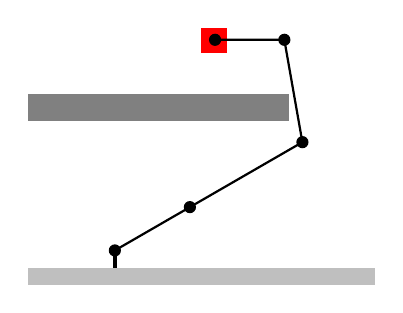
\begin{tikzpicture}[scale=1.1]
\coordinate (j1) at (1,0);
\fill[gray!50] (0,-2mm) rectangle +(4,-2mm);
\draw[very thick] (j1) -- +(0,-2mm);
\draw[fill,gray] (0,15mm) rectangle +(30mm,3mm);
\draw[red,fill] (57pt,65pt) rectangle +(8pt,8pt);
%\draw (0,0) -- (1,0) coordinate (j1)-- (4,0);
\draw[thick] (j1) -- ++(30:10mm) coordinate (j2) -- ++(30:15mm) coordinate (j3) -- ++(100:12mm) coordinate (j4) -- ++(180:8mm) coordinate (ee);
\fill (j1) circle [radius=2pt];
\fill (j2) circle [radius=2pt];
\fill (j3) circle [radius=2pt];
\fill (j4) circle [radius=2pt];
\fill (ee) circle [radius=2pt];
\end{tikzpicture}
}
\hspace{\fill}
\rightfigure{
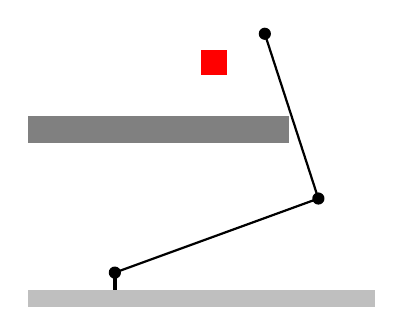
\begin{tikzpicture}[scale=1.1]
\coordinate (j1) at (1,0);
\fill[gray!50] (0,-2mm) rectangle +(4,-2mm);
\draw[very thick] (j1) -- +(0,-2mm);
\draw[fill,gray] (0,15mm) rectangle +(30mm,3mm);
\draw[red,fill] (57pt,65pt) rectangle +(8pt,8pt);
%\draw (0,0) -- (1,0) coordinate (j1)-- (4,0);
\draw[thick] (j1) -- ++(20:25mm) coordinate (j2) -- ++(108:20mm) coordinate (ee);
\fill (j1) circle [radius=2pt];
\fill (j2) circle [radius=2pt];
\fill (ee) circle [radius=2pt];
\end{tikzpicture}
}
\leftcaption{Arm with four actuators can reach a hidden position}\label{fig.redundant1}
\rightcaption{Arm with two actuators is blocked by an obstacle}\label{fig.redundant2}
\end{figure}

An important advantage of redundant systems arises from actuators with different characteristics. The mobile robot in Fig.~\ref{fig.hi-act-low-dof-2} can approach the target quickly, although its final position might not be accurate because of errors like uneven terrain. Once the mobile robot stops, the motors in the joints which do not have to deal with the terrain can be precisely positioned. While the positioning is precise, these joints do not have the broad range of the mobile base.

\subsubsection*{An example of a system with more actuators than DOF}

Figure~\ref{fig.act-dof} (top and side views) shows a configuration with \emph{two actuators and one DOF}. The system models a robotic crane that moves a heavy weight to a specific vertical position. Figure~\ref{fig.crane} shows a crane built from a Thymio robot and \lego{} components.\footnote{The winch is on the right of the robot not the left as in Fig.~\ref{fig.act-dof}.}

\begin{figure}
\begin{center}
\begin{tikzpicture}[align=left]
%
% Top view
%
\begin{scope}[scale=2.3,xshift=25mm]
% Table
\draw[fill,gray!20] (-34mm,-26mm) rectangle +(40mm,30mm);
% Robot
\draw (0,0) to [rounded corners] (-20mm,0) to [rounded corners, bend right=45] (-20mm,-18mm) to (0,-18mm) to cycle;
% Drive wheels
\fill (-11mm,0) rectangle +(8mm, 2mm);
\fill (-11mm,-18mm) rectangle +(8mm, -2mm);
\node at (-12mm,-8mm) {\p{driven wheels}};
\draw[->] (-8mm,-6mm) -- +(0,14pt);
\draw[->] (-8mm,-10mm) -- +(0,-20pt);
% Road wheels
\fill[gray!70] (-3mm,0) rectangle +(10mm, 2mm) node[above left,black,xshift=-38pt,yshift=13pt] {\p{road wheel}};
\draw[->] (1mm,5mm) -- +(0,-8pt);
\fill[gray!70] (-3mm,-23mm) rectangle +(10mm, -2mm);
\draw[fill,cyan] (2mm,0) rectangle +(2pt,-23mm);
\draw[fill,cyan] (2mm,-9mm) rectangle +(-4mm,2pt);
\draw[raxis] (2.4mm,-25.6mm) -- +(0,29mm);
% Winch
\fill[red] (-9mm,-20mm) rectangle +(4mm, -2mm) node[below left,black,xshift=-18pt,yshift=-7pt] {\p{winch}};
\draw[->] (-8mm,-25mm) -- +(0,8pt);
\draw[raxis] (-7mm,-24mm) -- +(0,27mm);
% Weight
\fill[red] (-41.1mm,-22mm) rectangle +(1.5mm,2mm);
% Bearing
\fill[gray!70] (-40mm,-22.8mm) rectangle +(2mm,4mm) node[above,xshift=-4mm,black,yshift=6pt] {\p{bearing and}\\\p{weight}};
\draw[raxis] (-39mm,-23.8mm) -- +(0,6mm);
% Cable
\draw[thick,red] (-9mm,-21mm) -- ++(-32mm,0);
\end{scope}
%
% Side view
%
\begin{scope}[yshift=-10.5cm]
% Table
\draw[fill,gray!20] (-2,-23.5mm) rectangle +(9.5,2mm);
\draw[fill,gray!20] (-1,-23.5mm) rectangle +(4mm,-15mm);
\draw[fill,gray!20] (5,-23.5mm) rectangle +(4mm,-15mm);
% Big wheel
\draw[fill,gray!70] (62mm,-9mm) circle[radius=1.25] node[left,black,xshift=-34pt,yshift=-8pt] {\p{road wheel}};
% Attachment
\draw[fill,cyan] (62mm,-9mm) circle[radius=4pt];
\draw[fill,cyan] (61.5mm,-9mm) rectangle +(3pt,20.5mm);
\draw[fill,cyan] (62.5mm,11mm) rectangle +(-5mm,3pt);
% Axis intersection of big wheel
\draw[raxis] (62mm,-9mm) -- +(24pt,0);
\draw[raxis] (62mm,-9mm) -- +(-24pt,0);
\draw[raxis] (62mm,-9mm) -- +(0,24pt);
\draw[raxis] (62mm,-9mm) -- +(0,-24pt);
% Robot
\draw[rounded corners,fill=white] (.2,0) -- (.2,2) -- (5.9, 2) -- (5.9,0) -- cycle;
% Wheel
\draw[fill,black] (4.3,9pt) circle[radius=1] node[left,black,xshift=-24pt,yshift=23pt] {\p{driven wheel}};
% Winch
\draw[fill,red]  (4.3,9pt) circle[radius=.5] node[above right,black,xshift=5pt,yshift=28pt] {\p{winch}};
\draw[->] (5,39pt) -- +(-16pt,-24pt);
\draw[raxis] (4.3,9pt) -- +(14pt,0);
\draw[raxis] (4.3,9pt) -- +(-14pt,0);
\draw[raxis] (4.3,9pt) -- +(0,14pt);
\draw[raxis] (4.3,9pt) -- +(0,-14pt);
% Support
\draw[fill,gray!70] (.9,0) rectangle +(.8,-17.5mm);
\draw[fill,gray!70] (.9,-17.5mm) arc(180:360:4mm);
% Bearing
\draw[red,fill=gray!70] (-85pt,13pt) circle[radius=10pt] node[above,black,yshift=4mm] {\p{bearing}};
\draw[thick,red] (4.3,23pt) -- (-85pt,23pt);
\draw[raxis] (-85pt,13pt) -- +(8pt,0);
\draw[raxis] (-85pt,13pt) -- +(-8pt,0);
\draw[raxis] (-85pt,13pt) -- +(0,8pt);
\draw[raxis] (-85pt,13pt) -- +(0,-8pt);
% Weight
\draw[thick,red] (-95pt,13pt) -- ++(0,-100pt);
\draw[fill,red] (-101pt,-95pt) rectangle +(12pt,12pt) node[right,black] {\p{weight}};
\end{scope}
\end{tikzpicture}
\caption{Robotic crane built from a mobile robot and a winch (top view above, side view below); in the side view the left wheel is not shown}\label{fig.act-dof}
\end{center}
\end{figure}

\begin{figure}
\begin{center}
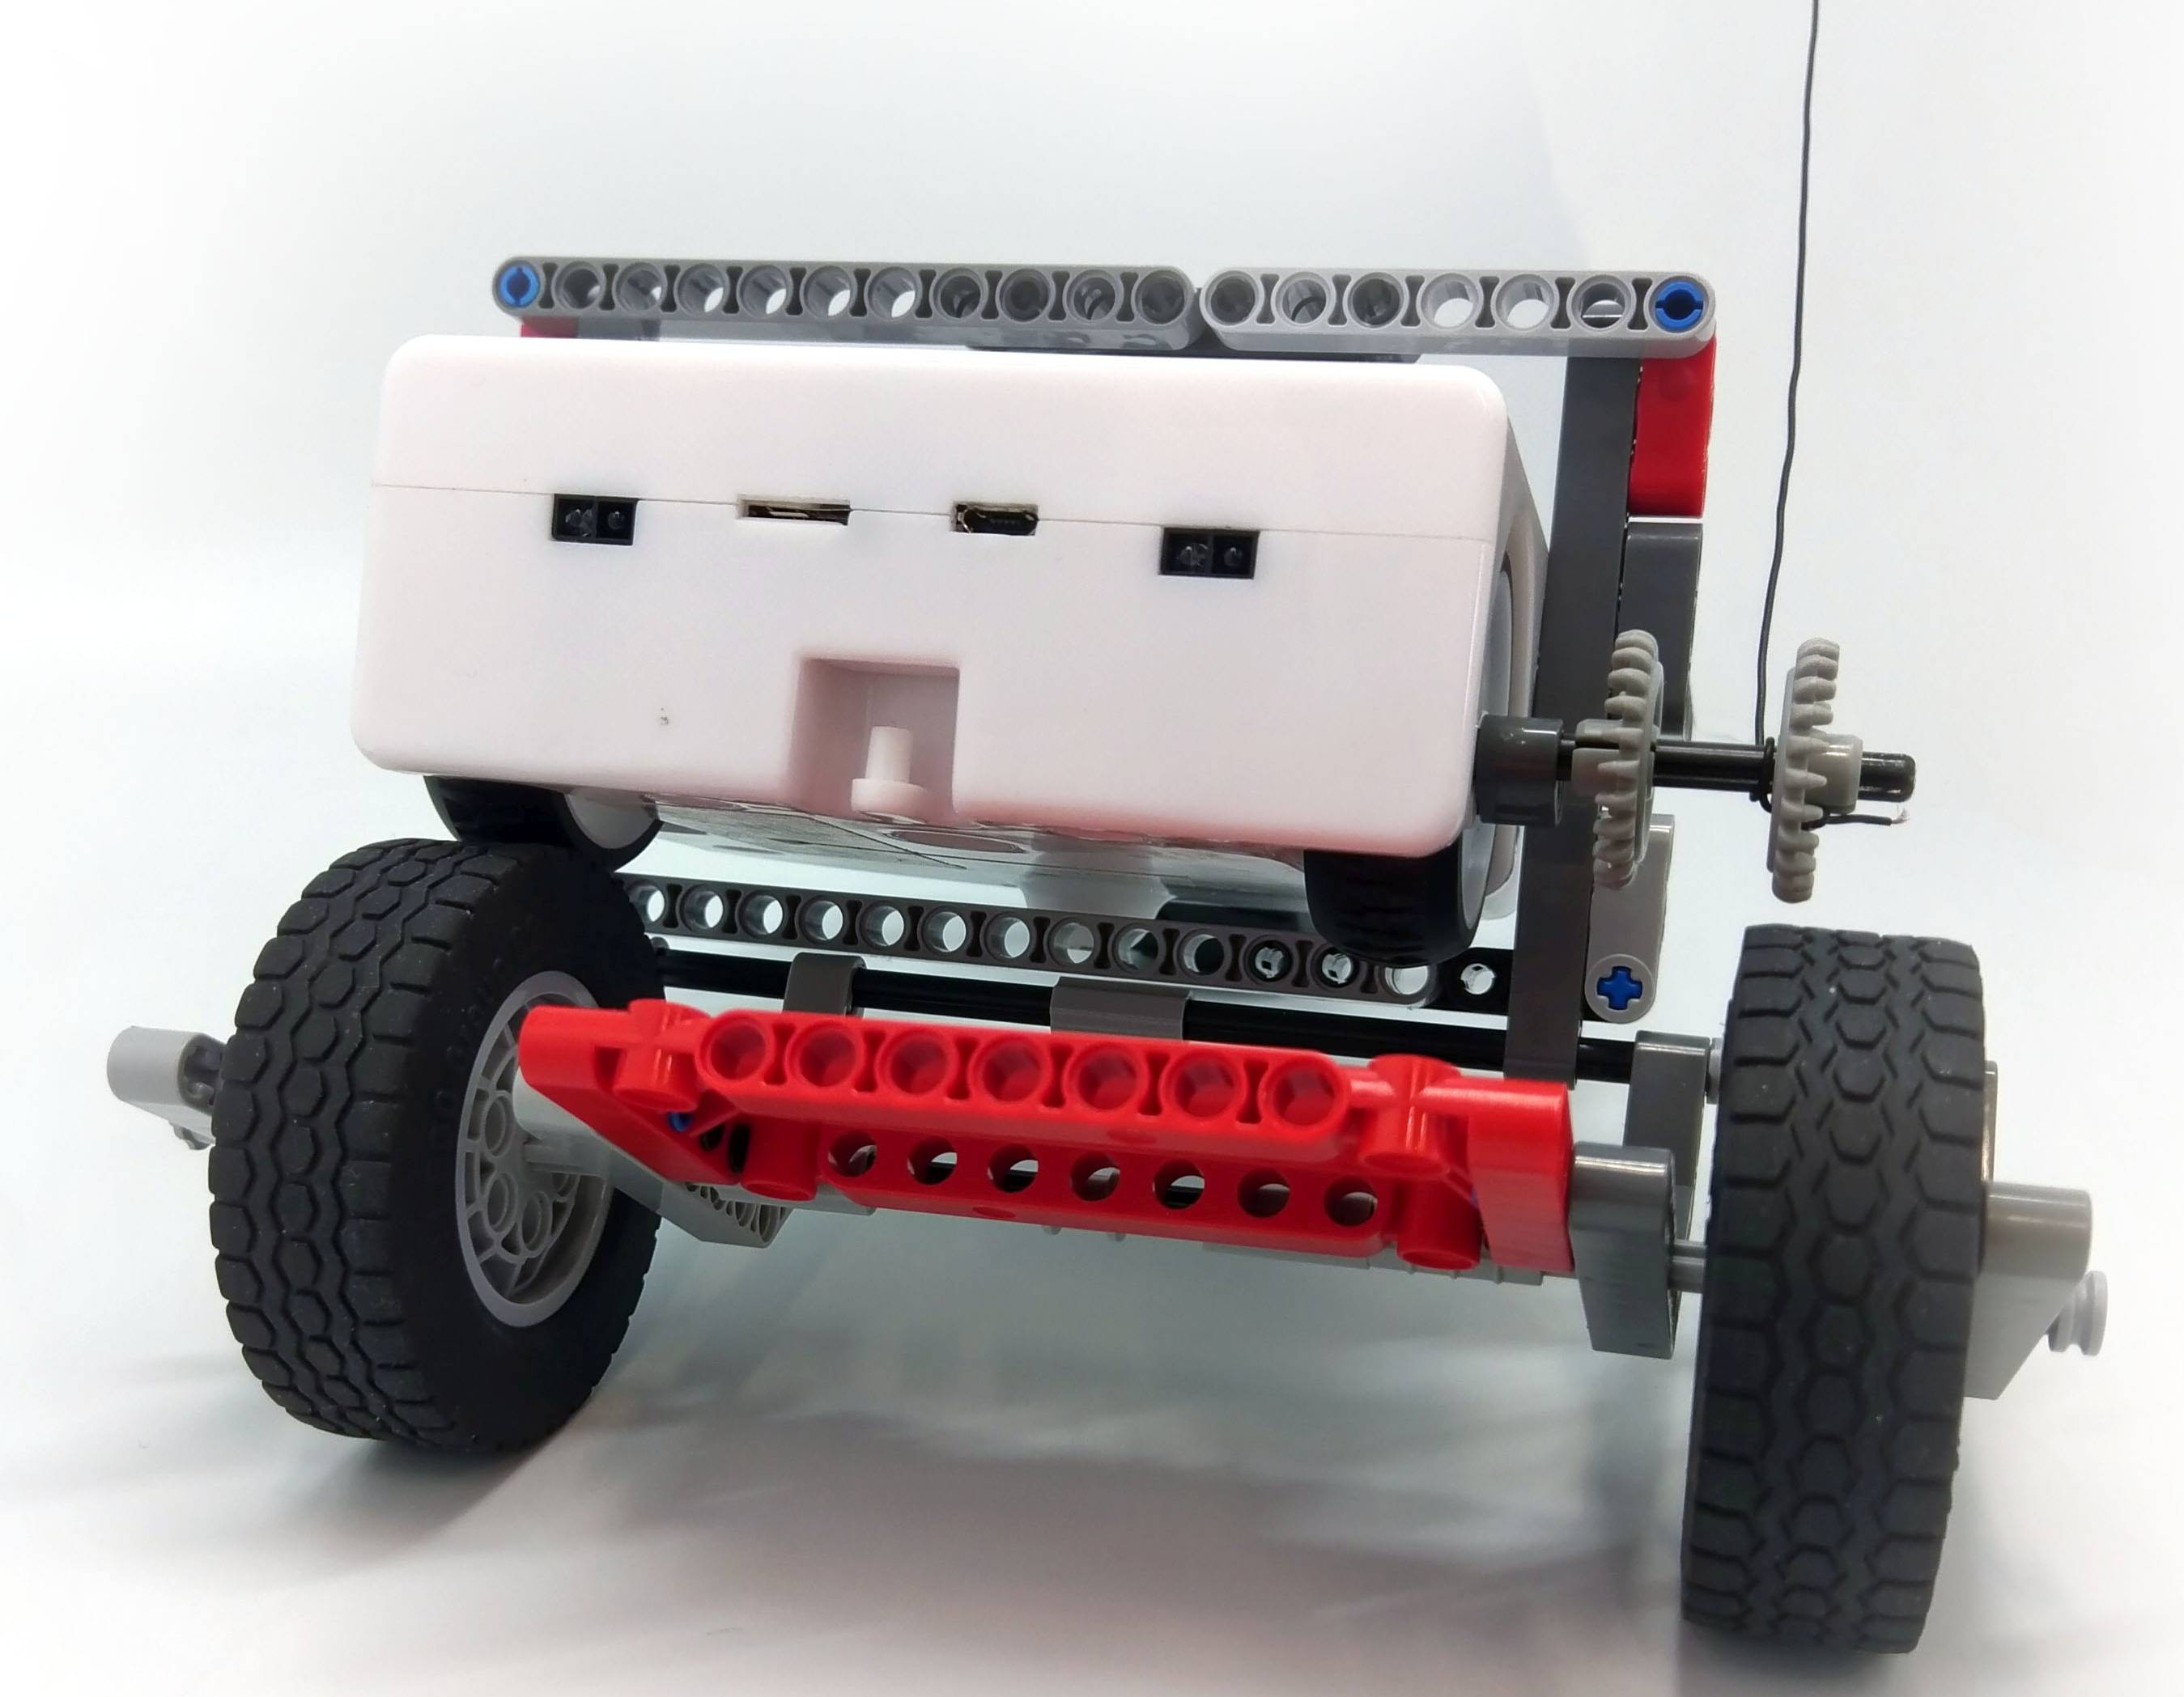
\includegraphics[width=.8\textwidth]{robotic-crane.jpg}
\caption{Robotic crane built from a Thymio robot and \lego{} components}\label{fig.crane}
\end{center}
\end{figure}

The system is build from a mobile robot with differential drive, but the wheels are not directly used to control the motion of the system. Instead, each wheel is an independent actuator. (Recall that the power to each wheel of a differential drive robot can be set independently to any value in a range such as $-100$ to $100$.)

The robot faces left. The right driven wheel in Fig.~\ref{fig.act-dof} (the black rectangle at the top of the top view and hidden behind the robot in the side view) controls a pair of (gray) road wheels that move the robot rapidly forwards and backwards. In turn, this causes the cable to move the weight rapidly up and down.

The road wheels are mounted on a structure (in blue) that is fixed to the robot body. There are several options for transferring power from the right driven wheel to the road wheels: friction, pulleys and belts, and gears. Each option has its own advantages and disadvantages, and all three are used in cars: the clutch uses friction, belts are used for timing and to run auxiliary components like water pumps, and gears are used in the transmission to control the torque applied to each wheel.

The left driven wheel (the black rectangle at the bottom of the top view and at the front of the side view) controls a winch (red) that rolls or unrolls a cable attached to the weight that moves up or down over a fixed bearing. The winch  has a diameter much smaller than the diameter of the driven wheels, so it can move the weight in small increments as the left driven wheel rotates. The design goal is to be able to perform precise positioning of the weight even though the winch moves the cable at a much slower speed than does the robot body.

There are two activities for this section. This activity is for readers who have good construction skills and an appropriate robotics kit. The second activity suggests alternate ways of demonstrating the concept of two actuators in one DOF.

\begin{framed}
\act{Robotic crane}{act-dof}
\begin{itemize}
\item Construct the robotic crane shown in Fig.~\ref{fig.act-dof}. Explain your choice of mechanism for connecting the driven wheel to the road wheels.
\item Write a program that given the current position of the weight and a goal position moves the weight to the goal position. Alternatively, send commands to the motors using a remote control device or a computer connected to the robot. \item Experiment with the relative rotational speeds of the left and right driven wheels that control the road wheels and the winch, respectively. Should you move the two actuators separately or simultaneously?
\end{itemize}
\end{framed}

\begin{framed}
\act{Robotic crane (alternatives)}{act-dof-alt}
\begin{itemize}
\item Write a program that causes a mobile robot to move forwards and backwards. Place a piece of black tape relatively far from the initial position of the robot. The goal is to cause the robot to stop as near as possible to the start of the tape \emph{without} continuously checking the sensor. 
\item The program has three modes of operation. (1) The robot moves fast, checking its sensor occasionally, and stopping when it detects the tape. (2) As in (1) but the robot moves slowly, checking its sensor relatively often. (3) As in (1) but when the tape is detected, the robot moves backwards using the speed and sampling period as in (2).
\item Run the program and compare the results of the three modes: the time until the robot stops and error between the robot's final position and the start of the tape.
\item Alternatively, run the program with the three modes on a computer and experiment with the motion parameters and the sampling periods. You will need to choose a model for the motion: constant velocity, constant acceleration, or (more realistically) acceleration then constant velocity and finally deceleration when the tape is detected.
\end{itemize}
\end{framed}

%%%%%%%%%%%%%%%%%%%%%%%%%%%%%%%%%%%%%%%%%%%%%%%%%%%%%%%%%%%


\section{Holonomic and non-holonomic motion}\label{s.holonomic}
\index{holonomic motion}

Section~\ref{s.dof} presented the concept of degree of freedom (DOF) and the role of the number of actuators. There is another concept that links the DOF and the actuators in the case of mobile robot: the \emph{degree of mobility (DOM)}\index{degree of mobility}. The degree of mobility $\delta_m$ corresponds to the number of degrees of freedom that can be \emph{directly accessed} by the actuators. A mobile robot in the plane has at most three DOF ($(x,y)$ position and heading), so the maximal degree of mobility of a mobile robot is $\delta_m = 3$.

Let consider the DOM of various vehicles. A train has one DOF because it can only move forwards along the tracks, and it has one actuator, its engine, that directly affects this single degree of freedom. Therefore, a train has a degree of mobility of $\delta_m = 1$, meaning that the single DOF can be directly accessed by the actuator.

A robot with differential drive has three DOF. The two actuators are the two motors which act on the wheels. They can directly access two DOF: (a) if both wheels turn at the same speed, the robot moves forwards or backwards; (b) if the wheels have speeds in opposite directions, the robot rotates in place. Therefore, we can directly access the DOF along the forward axis of translation and the DOF of the heading, but we cannot directly access the DOF of the lateral axis of translation (Fig.~\ref{fig.mobility-example1}). A differential drive mobile robot has a degree of mobility $\delta_m = 2 < 3 = \#\textrm{DOF}$.

\begin{figure}
\subfigures
\leftfigure
{
\begin{tikzpicture}[align=left,scale=.9]
\coordinate (origin) at (0,0);
\pic[scale=2.2] at (origin) {robot};
\draw[<-,thick] ($(origin)+(4pt,20pt)$) arc (90:-90:20pt);
\draw[->,thick] ($(origin)+(10pt,0)$) -- +(95pt,0);
\node at (18mm,-9mm) {\p{accessible}\\\p{DOF}};
\draw[->] (18mm,-5mm) -- +(0,4mm);
\draw[->] (15mm,-5mm) -- +(-5mm,2mm);
\draw[->,thick,dashed] ($(origin)+(0,5pt)$) -- +(0,85pt);
\node at (18mm,26mm) {\p{non-accessible}\\\p{DOF}};
\draw[->] (6mm,26mm) -- +(-5mm,0);
\end{tikzpicture}
}
\hspace{\fill}
\rightfigure
{
\begin{tikzpicture}[baseline=-20pt,align=left,scale=1.2]
\draw[rounded corners] (0,0) -- ++(4,0) -- ++(0,2) -- ++(-4,0) -- cycle;
\draw[rounded corners] (.5,.5) -- ++(1.5,0) -- ++(0,1) -- ++(-1.5,0) -- cycle;
\draw (.1,.1) -- (.5,.5);
\draw (.1,1.9) -- (.5,1.5);
\draw (2.4,.1) -- (2,.5);
\draw (2.4,1.9) -- (2,1.5);
\draw (2.5,.1) -- +(0,1.8);
\draw[<-,thick,dashed] (2.8,1.5) arc (90:-90:15pt);
\draw[->,thick] (3,1) -- +(45pt,0);
\draw[->,thick,dashed] (1.25,1) -- +(0,50pt);
\draw[fill,rotate around={30:(3.4,-.1)}] (3,-.2) rectangle +(.8,.2);
\draw[fill,rotate around={30:(3.4,2.1)}] (3,2) rectangle +(.8,.2);
\draw[fill] (.3,-2mm) rectangle +(.8,2mm);
\draw[fill] (.3,2) rectangle +(.8,2mm);
\node at (22mm,-4mm) {\p{accessible}\\\p{DOF}};
\draw[->] (26mm,-1mm) -- +(11mm,10mm);
\node at (26mm,25mm) {\p{non-accessible}\\\p{DOF}};
\draw[->] (17mm,24mm) -- +(-4mm,0);
\draw[->] (25mm,23mm) -- +(4mm,-7mm);
\draw[raxis] (.7,-6mm) -- +(0,10mm);
\draw[raxis] (.7,16mm) -- +(0,10mm);
\draw[raxis] (3.4,-.1) -- +(120:4mm);
\draw[raxis] (3.4,-.1) -- +(300:4mm);
\draw[raxis] (3.4,2.1) -- +(120:4mm);
\draw[raxis] (3.4,2.1) -- +(300:4mm);
\end{tikzpicture}
}
\leftcaption{Accessible and non-accesible DOF for a robot with differential drive}\label{fig.mobility-example1}
\rightcaption{Accessible and non-accesible DOF for a robot with Ackermann steering}\label{fig.mobility-example2}
\end{figure}

A car, like a robot with differential drive, has only two actuators for three DOF: one actuator, the motor, gives direct access to the degree of freedom along the longitudinal axis of the car, enabling it to move forwards and backwards. The other actuator, the steering wheel, does \emph{not} give direct access to any additional DOF, it can only orient the first DOF. The car cannot rotate around the vertical axis and it cannot move laterally (Fig.~\ref{fig.mobility-example2}). Therefore, a car has only one degree of mobility, $\delta_m = 1$. Intuitively, you can see the lower degree of mobility of a car compared with a robot with differential drive by noting that the robot can rotate in place while the car cannot.

By itself, a standard wheel has $\delta_m=2$: it can roll forwards and backwards and it can rotate around the vertical axis that goes through the point of contact of the wheel with the ground. A wheel cannot move sideways, which is actually a good thing because it prevents the vehicle from skidding off the road during a turn. In the car, the degree of mobility is reduced even further to $\delta_m=1$, because there are two pairs of wheels, one in the front and one in the rear of the car. This configuration makes it impossible for the car to rotate around its vertical axis, even though the individual wheels can do so (usually only the front wheels). The limitation to $\delta_m=1$ gives stability to the car---it cannot skid laterally and it cannot rotate---making it easy and safe to drive at high speeds. In fact, an accident can occur when rain or snow reduce the friction so that the car can skid or rotate.

An autonomous mobile robot can profit if it has a greater DOM $\delta_m = 3$. To directly access the third DOF, the robot needs to be able to move laterally. One method is to have the robot roll on a ball or a castor wheel like an office chair. Another method is to use \emph{Swedish wheels}\index{Swedish wheel} (Fig.~\ref{fig.swheel}). A Swedish wheel is a standard wheel that has small free wheels along its rim so that it can move laterally, enabling direct access to the third DOF.

\begin{figure}
\subfigures
\leftfigure
{
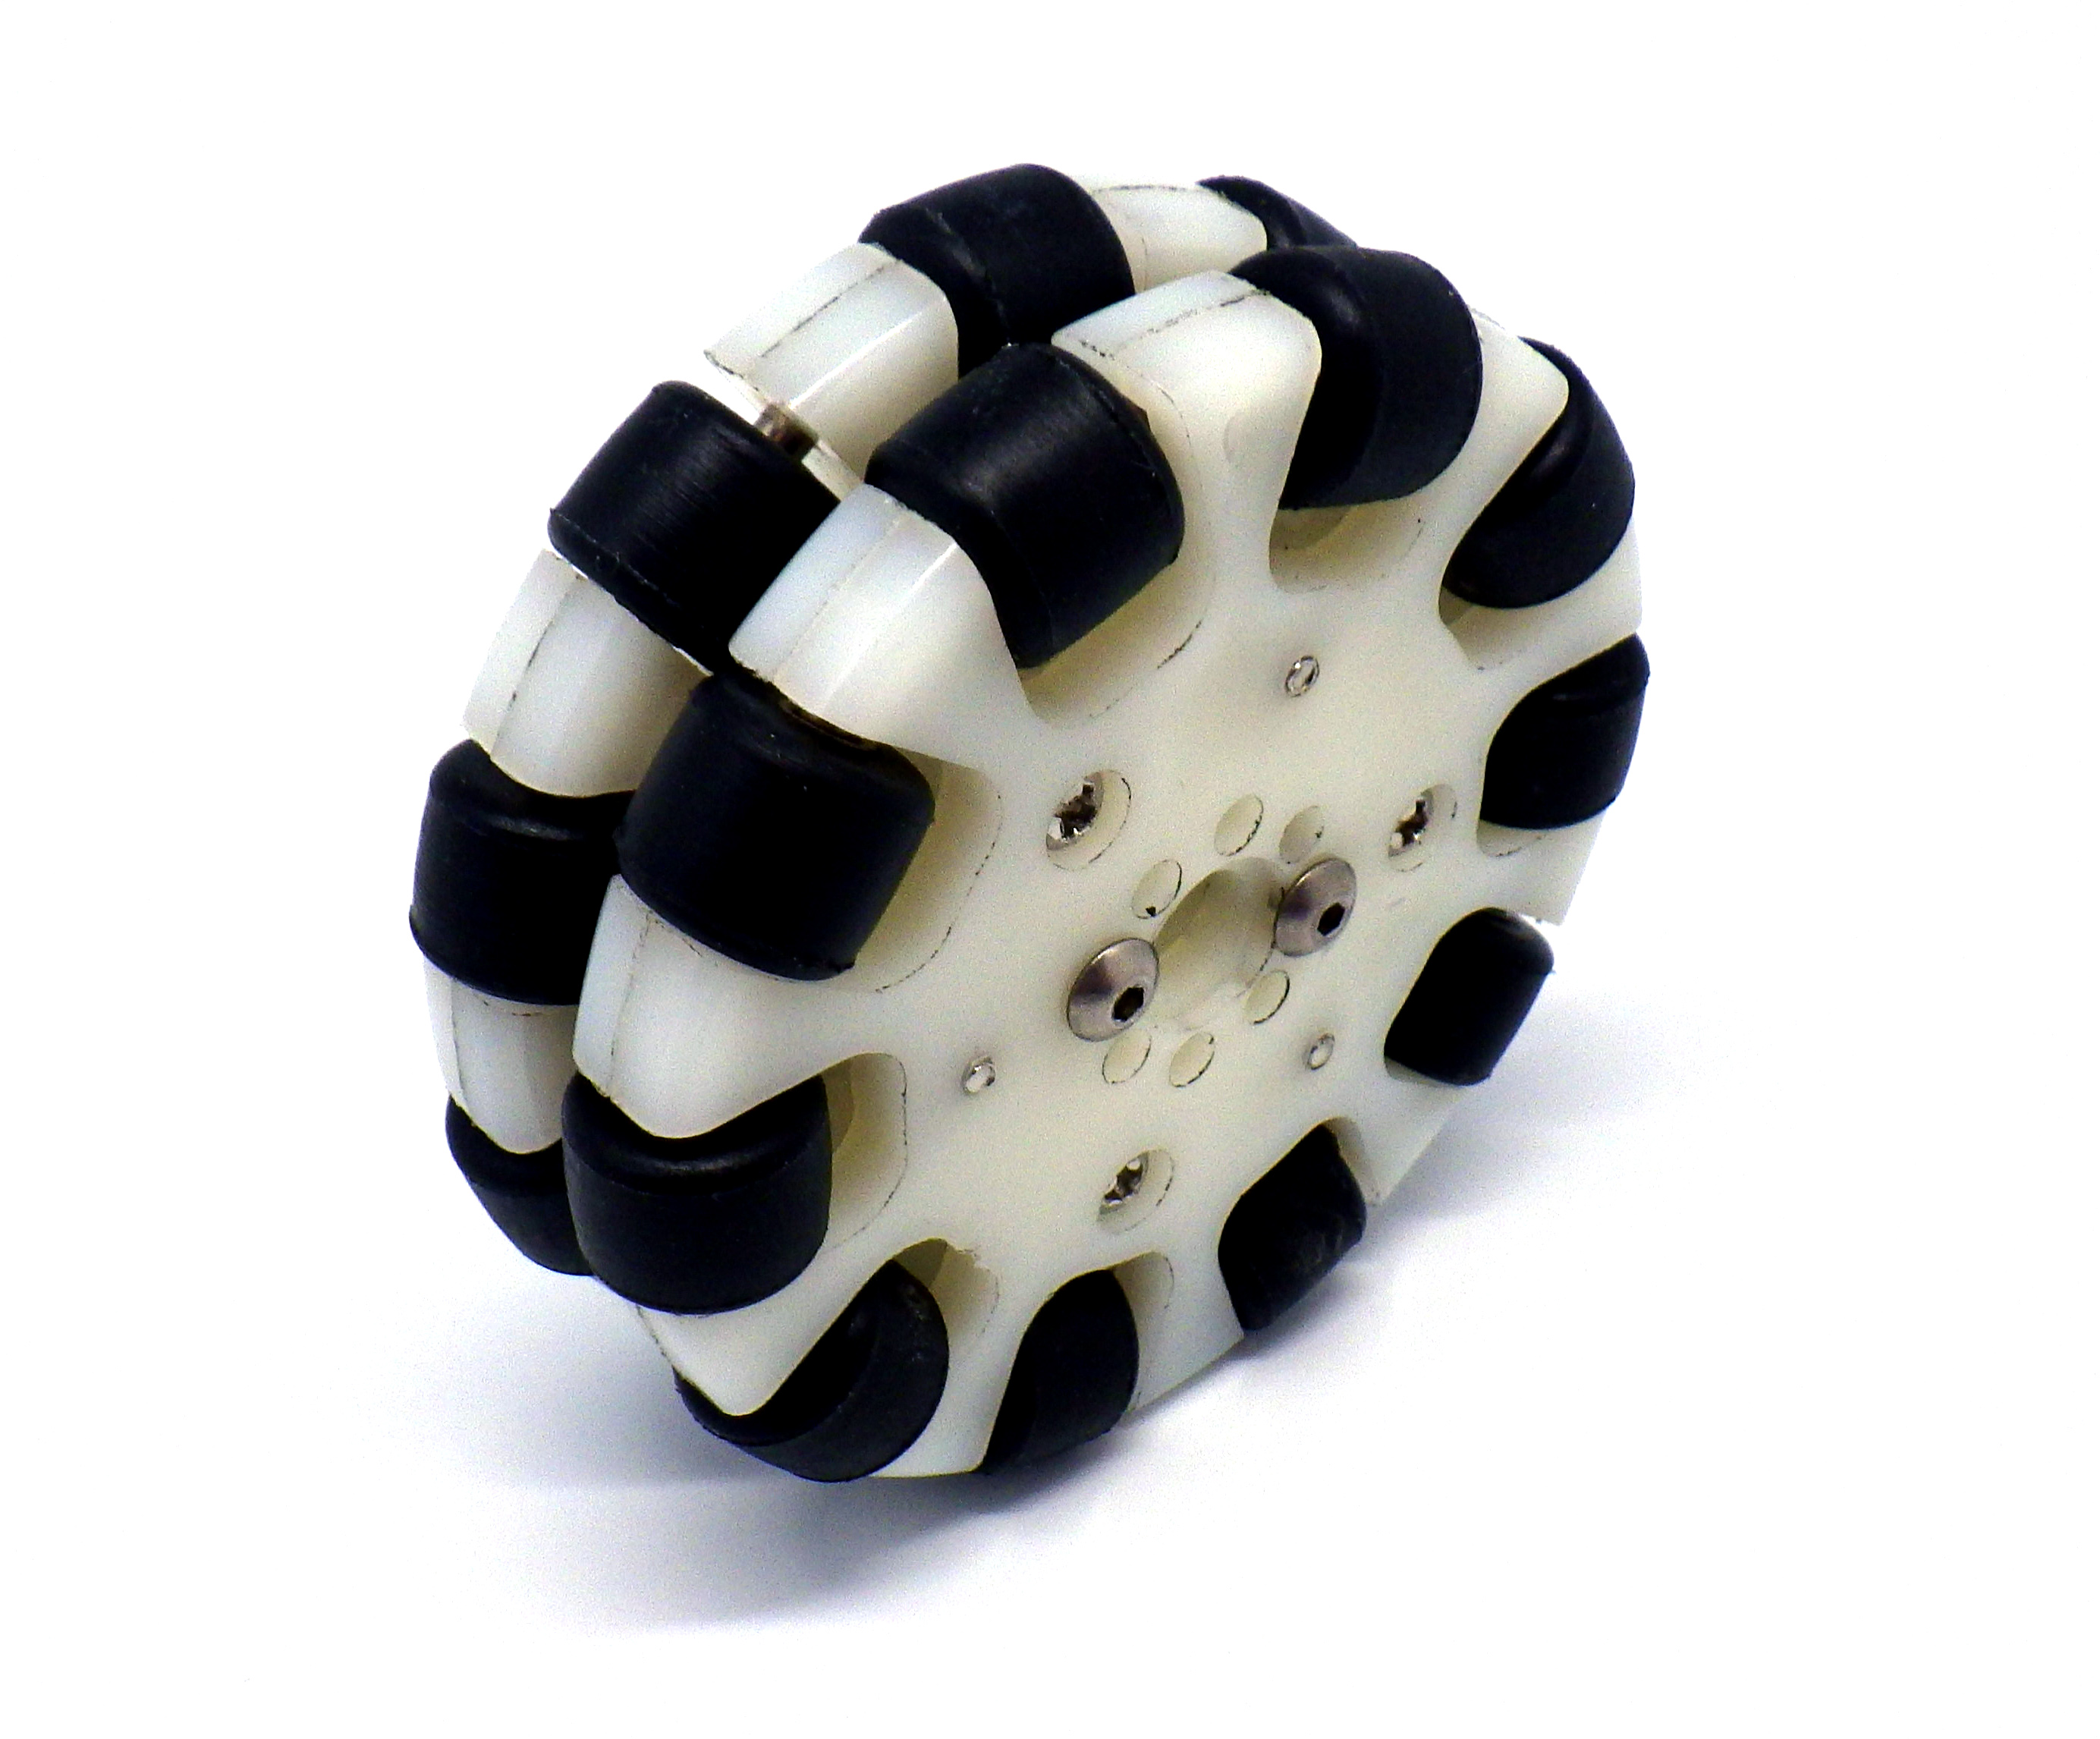
\includegraphics[width=0.45\textwidth]{omni-dir-wheel.jpg}
}
\hspace{\fill}
\rightfigure
{
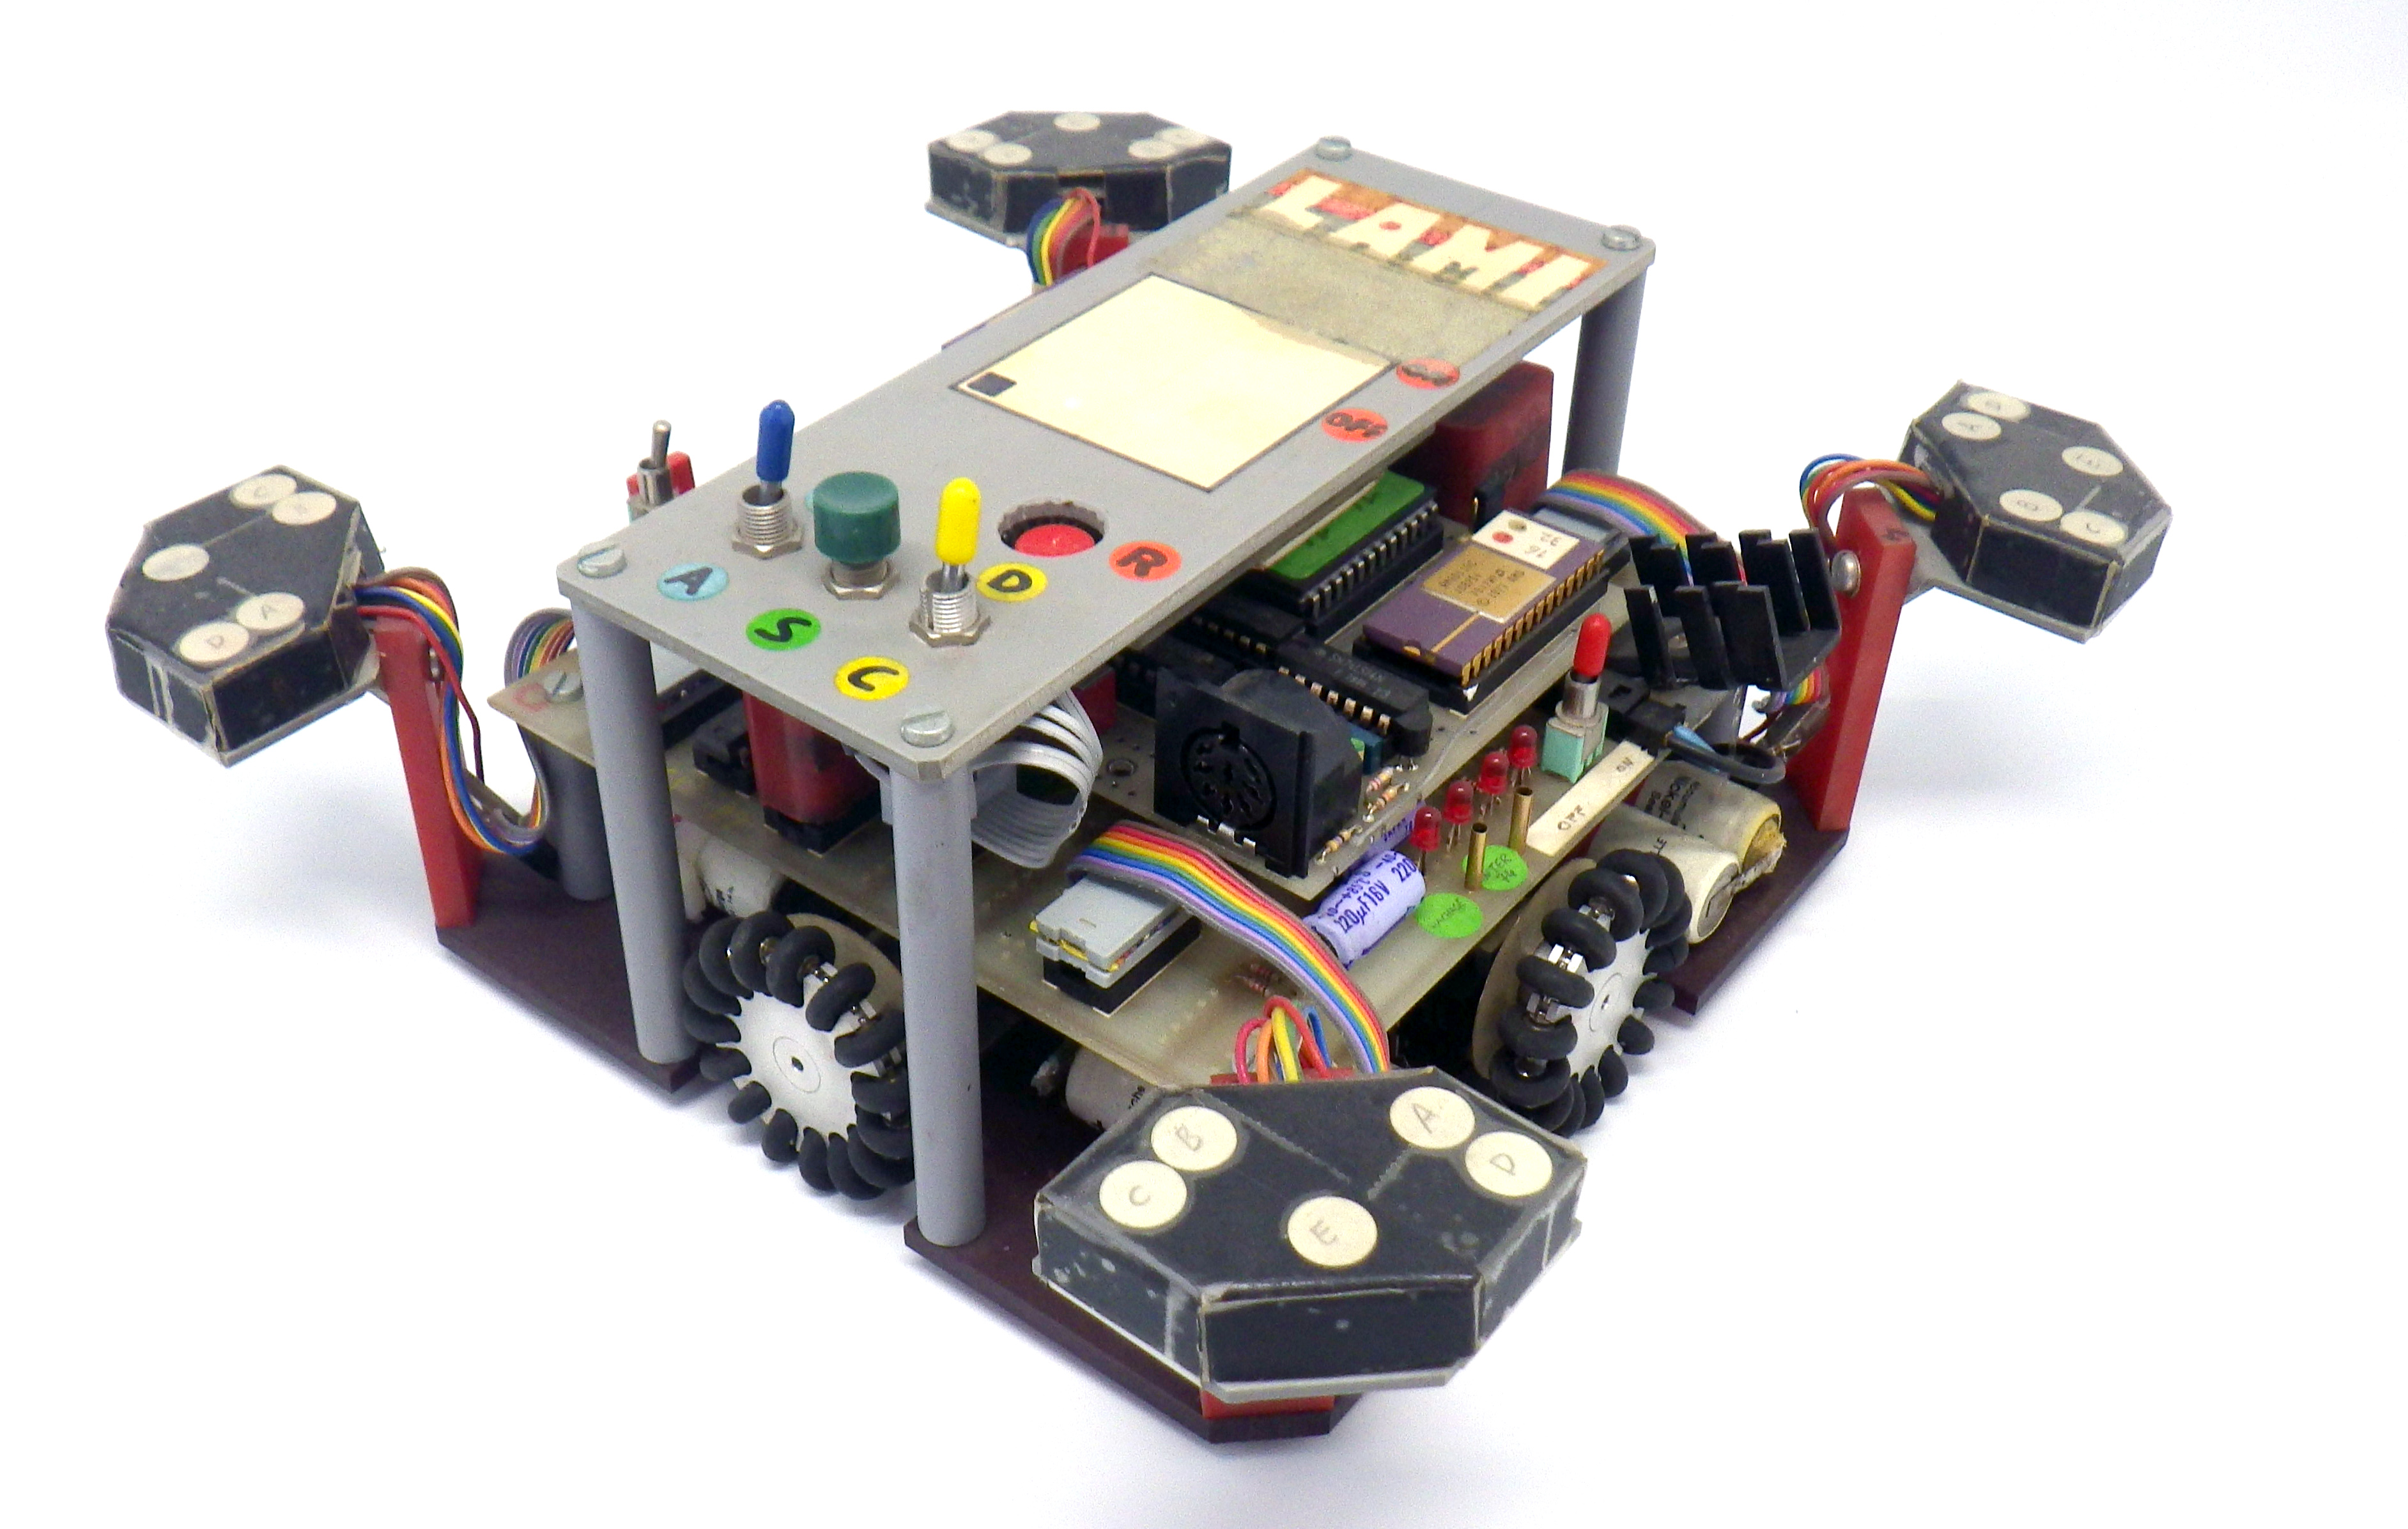
\includegraphics[width=0.5\textwidth]{omnirobot.jpg}
}
\leftcaption{Swedish wheel}\label{fig.swheel}
\rightcaption{Omnidirectional robot (Courtesy LAMI-EPFL)}\label{fig.omni-robot}
\end{figure}

Mobile robots that can directly access all three DOF ($\delta_m=3$) are called \emph{omnidirectional robots}\label{omnidirectional robot}. Figure~\ref{fig.omni-robot} shows an omnidirectional robot constructed with four Swedish wheels. The two pairs of wheels on opposite sides of the robot can directly move the robot left, right, forwards and backwards. This configuration is redundant but very easy to control. To avoid redundancy, most omnidirectional robots have three Swedish wheels mounted at an angle of $120^\circ$ from each other (Figh.~\ref{fig.omni3}). This configuration has $\delta_m=3$ but is not easy to control using the familiar $x,y$ coordinates.

\begin{figure}
\begin{center}
\begin{tikzpicture}[scale=0.8]
% Draw body of robot
\draw[fill,gray!20] (0,0) circle [radius=50pt];
% Draw three Swedish wheels
\foreach \r/\x/\y in {0/0/0,120/0cm/0cm,-120/0cm/0cm} {
	\begin{scope}[xshift=\x,yshift=\y,rotate=\r]
		% Draw axle
		\draw[thick,fill,gray] (-3,-0.1) rectangle +(-.5,.2);
		% Draw motor
		\draw[thick] (-3,-.5) rectangle +(2,1);
		% Draw wheel
		\draw[rounded corners,thick,fill=gray!20] (-4,-1) to [bend right=10] ++(.5,0)
		       -- ++(0,2) to [bend right=10] ++(-.5,0) -- cycle;
		\foreach \i in {-.8,-.2,.4} {
		  \draw[rounded corners,fill=gray] (-3.85,\i) rectangle +(.2,.4);
	  }
	\end{scope}
}
% Draw axes
\foreach \r/\x/\y/\len in {60/0/0/4.5cm,180/0cm/0cm/6cm,-60/0cm/0cm/4.5cm} {
	\begin{scope}[xshift=\x,yshift=\y]
	  \draw[raxis] (0,0) -- +(\r:\len);
  \end{scope}
}
\draw[->] (-3.75,1) -- +(0,.5) node[right] {\p{driven motion}};
\draw[->,thick] (-4,0) -- +(-1,0) node[above,xshift=-2mm] {\p{free motion}};
\node[xshift=-1.6cm,yshift=.2cm] at (0,0) {\p{motor}};
\end{tikzpicture}
\end{center}
\caption{Omnidirectional robot with three Swedish wheels}\label{fig.omni3}
\end{figure}

The relative values of the DOF and the DOM of a robot define the concept of holonomic motion. A robot has \emph{holonomic motion}\index{holonomic motion} if $\delta_m = \#\textrm{DOF}$ and it has \emph{non-holonomic motion} $\delta_m < \#\textrm{DOF}$. A holonomic robot like the one in Fig.~\ref{fig.omni-robot} can directly control all its DOF without difficult maneuvers. Figure~\ref{fig.parallel-omni} shows how easy it is for the omnidirectional robot with Swedish wheels (Fig.~\ref{fig.omni3}) to perform parallel parking.

\begin{figure}
\begin{center}
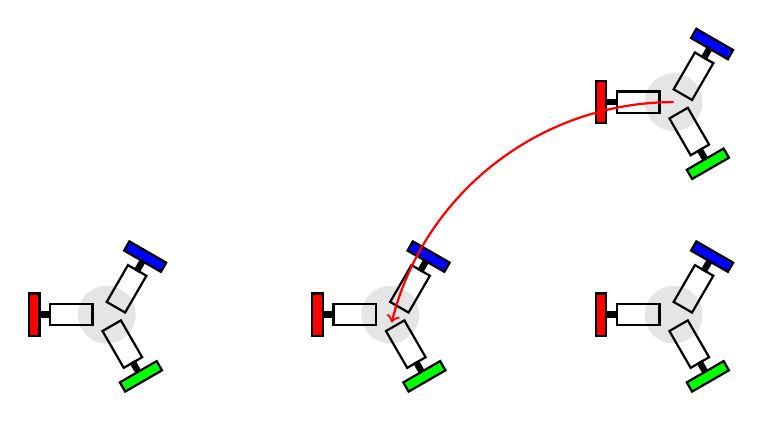
\begin{tikzpicture}[scale=.9]
\foreach \a/\b in {0/0,-40mm/-30mm,-80mm/-30mm,0/-30mm} {
	\draw[fill,gray!20] (\a,\b) circle [radius=4mm];
	\foreach \r/\x/\y/\color in {0/-8mm/-1.5mm/red,120/5mm/-6mm/green,-120/3mm/7mm/blue} {
		\begin{scope}[xshift=\x+\a,yshift=\y+\b,rotate=\r,scale=.3]
			% Draw axle
			\draw[thick,fill,gray] (0,.4) rectangle +(-.5,.2);
			% Draw motor
			\draw[thick] (0,0) rectangle +(2,1);
			% Draw wheel
			\draw[thick,fill=\color] (-1,-.5) to ++(.5,0)
	       -- ++(0,2) to ++(-.5,0) -- cycle;
		\end{scope}
	}
}
\draw[thick,red,->] (0,0) arc (90:166:41mm);
\end{tikzpicture}
\end{center}
\caption{Parallel parking by an omnidirectional robot}\label{fig.parallel-omni}
\end{figure}

A car and a robot with differential drive are non-holonomic because their DOM ($\delta_m=1$ and $\delta_m=2$, respectively) are lower than their DOF which is three. Because of this limited degree of mobility, these vehicles need complex steering maneuvers, for example, to perform parallel parking. There is a significant difference between the two vehicles. The differential drive robot needs three separate movements, but they are very simple (Fig.~\ref{fig.parallel-diff}): rotate left, move backwards, rotate right. The car also needs three separate movements, but they are extremely difficult to perform correctly (Fig.~\ref{fig.parallel-car}). You have to estimate where to start the maneuver, how sharp to make each turn and how far to move between turns. The higher DOM of the differential drive robot is advantageous in this situation.

\begin{figure}
\subfigures
\leftfigure{
\begin{tikzpicture}
\pic[scale=.5] at (-14mm,-4mm) { robot };
\pic[scale=.5] at (18mm,-4mm) { robot };
\pic[scale=.5] at (2mm,15mm) { robot };
\pic[rotate=90,scale=.5] at (2mm,15mm) { robot };
\pic[scale=.5] at (2mm,-4mm) { robot };
\pic[rotate=90,scale=.5] at (2mm,-4mm) { robot };
\draw[->,thick,green!60!black] (2mm,10mm) -- +(0,-6mm);
\draw[thick,red,->] (2mm,-4mm) arc (180:90:5mm);
\draw[thick,blue,->] (2mm,15mm) arc (0:90:5mm);
\end{tikzpicture}
}
\hspace{\fill}
\rightfigure{
\begin{tikzpicture}
\pic[scale=.5] at (-14mm,-4mm) { car };
\pic[scale=.5] at (18mm,-4mm) { car };
\pic[scale=.5] at (20mm,15mm) { car };
\draw[thick,red,->] (18mm,15mm) arc (90:180:10mm);
\draw[thick,blue,->] (8mm,6mm) arc (0:-90:10mm);
\draw[thick,green!60!black,->] (-1mm,-4mm) -- (12mm,-4mm);
\end{tikzpicture}
}
\leftcaption{Parallel parking for a non-holonomic differential drive robot}\label{fig.parallel-diff}
\rightcaption{Parallel parking for a non-holonomic car}\label{fig.parallel-car}
\end{figure}

\begin{framed}
\act{Holonomic and non-holonomic motion}{holonomic}
\begin{itemize}
\item Look again at the mobile robot which is constrained to rotational motion only (Fig.~\ref{fig.rot-dof}). What is its degree of mobility $\delta_m$? It is holonomic or not?
\item Figure~\ref{fig.wallcleaning} shows a robot for cleaning the walls of a building. There are two anchors from which cables descend, passing through eyes fixed to the robot's body and then to winches powered by the robot's wheels. By rolling and unrolling the cables, the robot moves up and down the wall. However, if the two motors do not cause the wheels move precisely at the same rotational velocity, the robot will swing from side to side. How many DOF and how many DOM does this robot have? Is it holonomic or not?
\end{itemize}
\end{framed}


\begin{figure}
\begin{center}
\begin{tikzpicture}[scale=1.2]
% Robot
\pic[rotate=90,scale=1.3] at (0,0) { robot };
% Left and right
\foreach \sign in {1,-1} {
  % Winch
  \draw (\sign*8.5mm,-1mm) rectangle +(\sign*3mm,2mm);
  \draw[fill] (\sign*11.5mm,-2mm) rectangle +(\sign*1mm,4mm);
  % Cable on winch
  \foreach \x in {9mm,9.5mm,10mm,10.5mm,11mm} {
    \draw[red] (\sign*\x,-1mm) -- +(0mm,2mm);
  }
  % Cable
  \draw[red,thick] (\sign*10mm,0mm) -- (\sign*10.8mm,18.5mm) -- (\sign*30mm,45mm);
  % Eyes
  \draw (\sign*10.8mm,18.5mm) circle [radius=.8mm];
  % Anchors
  \draw[fill,gray] (\sign*30mm,45mm) circle [radius=1mm];
}
\draw[fill,gray] (-.5mm,10mm) rectangle +(1mm,8mm); 
\draw[fill,gray] (-10mm,18mm) rectangle +(20mm,1mm);
\node at (0,45mm) {\p{anchors}};
\draw[->] (6mm,45mm) -- +(20mm,0);
\draw[->] (-6mm,45mm) -- +(-20mm,0);
\begin{scope}[yshift=5mm]
\node at (-22mm,0mm) {\p{winch}};
\node at (22mm,0mm) {\p{winch}};
\draw[->] (-18mm,0mm) -- +(5mm,-2mm);
\draw[->] (18mm,0mm) -- +(-5mm,-2mm);
\end{scope}
\draw[raxis] (-18mm,0mm) -- (18mm,0mm);
\end{tikzpicture}
\end{center}
\caption{Robot for cleaning a wall}\label{fig.wallcleaning}
\end{figure}

\section{Summary}

A mobile robot like a self-driving car or a Mars explorer will not have landmarks always available for navigation. Odometry is used to bring the robot to the vicinity of its goal without reference to the environment. The robot estimates its speed and rotational velocity from the power applied to its motors. Odometry can be improved by using wheel encoders to measure the number of revolutions of the wheels, rather than inferring the velocity from the motor power. The change in the position of an inexpensive robot moving in a straight line can be computed by multiplying speed by time. If the robot is turning, trigonometric calculations are needed to compute the new position and orientation. Even with wheel encoders, odometry is subject to errors that can be very large if the error is in the heading.

Inertial navigation uses accelerometers and gyroscopes to improve the accuracy of odometry. Integrating acceleration gives velocity and integrating angular velocity gives the heading. Microelectromechanical systems have made inertial navigation inexpensive enough for use in robotics.

The DOF of a system is the number of dimensions in which it can move---up to three dimensions on a surface and up to six dimensions in the air or underwater---but a robot may be constrained to have fewer than the maximum number of DOF. An additional consideration is the number and configuration of the actuators of a robot which define its degree of mobility. If the DOM is equal to the number of DOF, the robot is holonomic and it can move directly from one pose to another, although it may be difficult to control. If the DOM is less than the number of DOF, the robot is non-holonomic; it cannot move directly from one pose to another and will require complex maneuvers to carry out some tasks.

\section{Further reading}

A detailed mathematical treatment of odometry errors in two dimensions is given in \cite[Sect.~5.24]{siegwart}. For an overview of inertial navigation see \cite{king,oxford}. Advanced textbooks on robotics present holonomy \cite{correll,craig,siegwart,spong}.

\bibliographystyle{spmpsci}
\bibliography{er}
